%% Template for EU deliverable, using the deliverable.sty style file

\documentclass[12pt,a4paper,twoside]{article}

%% common package
\usepackage[headers]{deliverable}
\usepackage{xspace}
\usepackage{verbatim}
\usepackage[usenames]{color}
\usepackage[usenames,dvipsnames]{xcolor}
\usepackage{graphicx}

\usepackage{url}
\usepackage{array}
\usepackage{amsmath,bm,amsfonts}
\usepackage{tikz}
\usetikzlibrary{arrows,automata}
\usepackage{IEEEtrantools}
\usepackage{mathtools}
\DeclareMathOperator*{\argmin}{argmin}
%
%
%\usepackage{times}
%
% numbers option provides compact numerical references in the text. 
\usepackage[numbers]{natbib}
\usepackage{multicol}
\usepackage[bookmarks=true]{hyperref}

\usepackage{graphicx,import}
\usepackage{mathtools, amssymb}
\usepackage{paralist}
\usepackage[pdf]{svg}
\usepackage{amsmath,amssymb,amsthm}

% \usepackage{mathptmx}      % use Times fonts if available on your TeX system
% insert here the call for the packages your document requires
%\usepackage{latexsym}
% etc.
% \usepackage{color}
\usepackage{graphicx} % for pdf, bitmapped graphics files
% \usepackage{float}
\usepackage{times}
% \usepackage{multicol}
% \usepackage{multirow}	% multi row for table
\usepackage{mathtools,amsfonts,amssymb,amsmath, bm}
% \usepackage{cases}
% \usepackage{enumerate}
\usepackage{caption}
\usepackage[font=small]{caption}
\usepackage{paralist}
% \usepackage{colortbl}
\usepackage{xparse}
\usepackage{float}
\usepackage{import}
\usepackage[mediumspace,mediumqspace,Grey,squaren]{SIunits}

%%%%%%%%%%%%%%%%%%%%%%%%%%%%%%%%%%%%%%%%%%%%%%%%%%%%%%%%%%%%%%%%%%%%%%%%%%%%%%%%%%%%%%%%%%%%%%%%
% please place your own definitions here and don't use \def but
% \newcommand{}{}
\newcommand{\fratop}[2]{\genfrac{}{}{0pt}{}{#1}{#2}}
\newcommand{\mx}[1]{\mathbf{\bm{#1}}} 				% Matrix symbol
\newcommand{\vc}[1]{\mathbf{\bm{#1}}} 					% Vector symbol
% \newcommand{\degree}{\ensuremath{^\circ}}				% define the degree symbol
\newcommand{\pder}[2]{\frac{\partial#1}{\partial#2}}		% partial derivative
\newcommand{\refframe}[1]{\mbox{\textless#1\textgreater}}	% to denote a reference frame
\DeclareMathOperator*{\argmax}{\arg\!\max}				% argmax
\DeclareMathOperator*{\dif}{\mathrm{d}}					% d
\DeclareMathOperator*{\half}{\frac{1}{2}}					% one half
\DeclareMathOperator{\sgn}{sgn}
\newcommand{\mat}[1]{\ensuremath{\begin{bmatrix}#1\end{bmatrix}}}	% matrix
\newcommand{\rank}[1]{\text{rank}\left(#1\right)}							% rank
\newcommand{\diag}[1]{\text{diag}\left(#1\right)}							% diag
\newcommand{\x}{\ensuremath{\times}}





% \pdfinfo{
%    /Author (Homer Simpson)
%    /Title  (Robots: Our new overlords)
%    /CreationDate (D:20160128120000)
%    /Subject ()
%    /Keywords (Robotics;)
% }

\newtheorem{assumption}{\bf{Assumption}}
\newtheorem{definition}{\bf{Definition}}
\newtheorem{boldLemma}{\bf{Lemma}}
%%

%%insert here other packages needed by sections

%%

%%%%%%%%%%%%%%%%%%%%%%%%%%%%%%%%%%%%%%%%%%%%%%%%%%%%%%%%%%%%%%%%%%%%%%%%%%%%%%
%%% Titlepage
%%%%%%%%%%%%%%%%%%%%%%%%%%%%%%%%%%%%%%%%%%%%%%%%%%%%%%%%%%%%%%%%%%%%%%%%%%%%%%

% declaration of variables used in style
\deliverableDocnumber{D5.4}
\deliverableTitle{Validation scenario 4: learning how to stand up with the help of a human caregiver.}

\deliverableAuthor{Francesco Nori}
\deliverableResponsiblePartner{IIT}
\deliverableAffiliation{% Insert here authors affiliations
 $^1$ IIT
}

\deliverableReviewer{Francesco Nori}
\deliverableCoordinator{Francesco Nori}
\deliverableActivityNumber{n} %% n=1,..,10
\deliverableActivity{RTD}
\deliverableDoctype{Deliverable} %% or Prototype
\deliverableClassification{Public} % or Consortium
\deliverableDistribution{Consortium} %
\deliverableStatus{Draft} % Draft or Final
\deliverableDeliveryDate{28/2/2017}
\deliverableFile{D5.4.pdf} % please do not use "-" in the name
\deliverableVersion{1.0}
\deliverableDate{Feb.~28, 2017}
\deliverableYear{2017}
\deliverablePages{\pageref{LastPage}}
\deliverableChangelog{v.1.0 & Feb 19, 2017 & First draft %%\\\hline
%%              v.2.0 & Feb 20, 2007 & Final version
}
\deliverableProjectStartingDate{1st March 2013}
\deliverableProjectEndDate{28th February 2017}
\deliverableProjectAcronym{CoDyCo}
\deliverableProjectTitle{Whole-Body Compliant Dynamical Contacts in Cognitive Humanoids}
 \deliverableContractNumber{600716}
 \deliverableProjectCoordinator{Istituto Italiano di Tecnologia}
 \deliverableProjectUrl{www.codyco.eu}
 \deliverableFrameworkProgramme{FP7}
 
 \deliverableWorkpackage{deliv WP5}
 \deliverableEditors{Francesco Nori}
 \deliverableContributors{Daniele Pucci, Francesco Romano, Jorhabib Eljaik, Silvio Traversaro, Vincent Padois, Francesco Nori, Claudia Latella, Marta Lorenzini, Maria Lazzaroni, Oriane Dermy, Serena Ivaldi, Alexandros Paraschos, Olivier Rochel}
 \deliverableReviewers{}
\deliverableAbstract{This deliverable discusses the technical details and choices for the implementation of the year-4 validation scenario of the CoDyCo project.  The validation scenario aims at validating the theoretical results in robot whole-body control while interacting with humans. Physical human-robot interaction is a field of growing interest among the scientific community. One of the main challenges is to replicate the physical mutual interaction occurring during human-human collaborative tasks. For this purpose, the knowledge about human whole-body motions and forces is mandatory but the current state of the art on robots ability in estimating them is not sufficient to yield to a suitable interaction. This deliverable presents a human-robot physical interaction task and exploits a wearable technology to monitor humans dynamics during the interaction}
\deliverableReviewers{}
\deliverableKeywordList{Whole-body human dynamics, Human-robot physical collaboration, Probabilistic sensor fusion algorithm}

%%%%%%%%%%%%%%%%%%%%%%%%%%%%%%%%%%%%%%%%%%%%%%%%%%%%%%%%%%%%%%%%%%%%%%%%%%%%%%
%%% Sections
%%%%%%%%%%%%%%%%%%%%%%%%%%%%%%%%%%%%%%%%%%%%%%%%%%%%%%%%%%%%%%%%%%%%%%%%%%%%%%


%%
%%%%%%%%%%%%%%%%%%%%%%%%%%%%%% BEGIN DOCUMENT
\begin{document}

\deliverableMaketitle

%%TODO move to style
\newcolumntype{L}[1]{>{\raggedright\let\newline\\\arraybackslash\hspace{0pt}}m{#1}}
\newcolumntype{C}[1]{>{\centering\let\newline\\\arraybackslash\hspace{0pt}}m{#1}}
\newcolumntype{R}[1]{>{\raggedleft\let\newline\\\arraybackslash\hspace{0pt}}m{#1}}

\textbf{Document Revision History}
\begin{center}
\begin{tabular}{|C{2cm}|C{3cm}|p{5cm}|C{4cm}|}
\hline
\textbf{Version}&\textbf{Date}&\textbf{Description}&\textbf{Author}\\\hline
First draft & 19 Feb 2017 & In this version we simply write down a few considerations on the fourth year validation scenario as discussed after the mid-year CoDyCo meeting in Nancy. & Francesco Nori \\\hline
\hline
Final version & 27 Feb 2017 & None & Francesco Nori \\\hline
\end{tabular}
\end{center}
 
 \clearpage

\newpage
\renewcommand*\contentsname{Table of Contents}
\renewcommand*\listfigurename{Index of Figures}
\tableofcontents
\newpage
\newpage

 

% \PACS{PACS code1 \and PACS code2 \and more}
% \subclass{MSC code1 \and MSC code2 \and more}

%%%%%%%%%%%%%%%%%%%%%%%%%%%%%%%%%%%%%%%%%%%%%%%%%%%%%%%%%%%%%%%%%%% SECTIONS
%!TEX root = ../template.tex

\section{Introduction}
%
The understanding of the human dynamics and the way in which its contribute
 can be applied to enhance a physical
 human-robot interaction (pHRI) are two of the most promising challenges for the scientific
  community due mainly to their enormous and to-be-developed potential in industrial scenarios,
   ergonomics context, as well as in assistive and rehabilitation fields. 
Classical robots are built to act \emph{for} humans, but in order to adapt their functionality
 to the current technological progress, the new generation of robots will have to collaborate
  \emph{with} humans.  This implies that the robots will be endowed with the capability to
   control physical collaboration through intentional interaction with humans.
To achieve this condition, robots have to know mandatorily the dynamics (contact forces, internal forces,
  joint torques) of
  the human agent who they are interacting with.  However the current state of the robot 
  knowledge in
   observing human whole-body dynamics  yields to non-proficient and unadaptive interactions.
   		\\	   	   
   \indent
  To overcome this drawback, it is fundamental to understand what
   the response of the human body is while a physical interaction is
    occurring.  The importance in retrieving this information is exemplified in Fig.
	 \ref{fig:figs_schemeFrameworkLoop}: once the dynamic variables are computed by 
	 exploiting a dynamics estimation algorithm, the human dynamics feedback 
	 may be provided to the robot
	   controllers. As a consequence, the robot may adjust the strategy of interaction accordingly.
		\\	   	   
\indent
This work is the first attempt to go in this direction since a first pHRI task was
 inserted with respect to our previous work \cite{LatellaSensors2016} where only an
  investigation on the human inverse dynamics was carried out. The paper is built on the
   theoretical framework described in \cite{LatellaSensors2016} from which it inherits 
   both the notation and formulation.
   \\  
   \indent
The paper is structured as follows.  Section $2$ introduces the state-of-the-art background 
which the paper is based on.  Section $3$ presents the modelling of the human
body as an articulated multi-body system. In Section $4$ the adopted
Gaussian probabilistic domain for the sensor fusion methodology is briefly recalled.  Section $5$ outlines the 
experimental set-up followed by a description of the results in Section $6$.  
Conclusions and several considerations on the pivotal role of further control and 
estimation developments are depicted in Section $7$.
%	
\begin{figure}[ht]
  \centering
   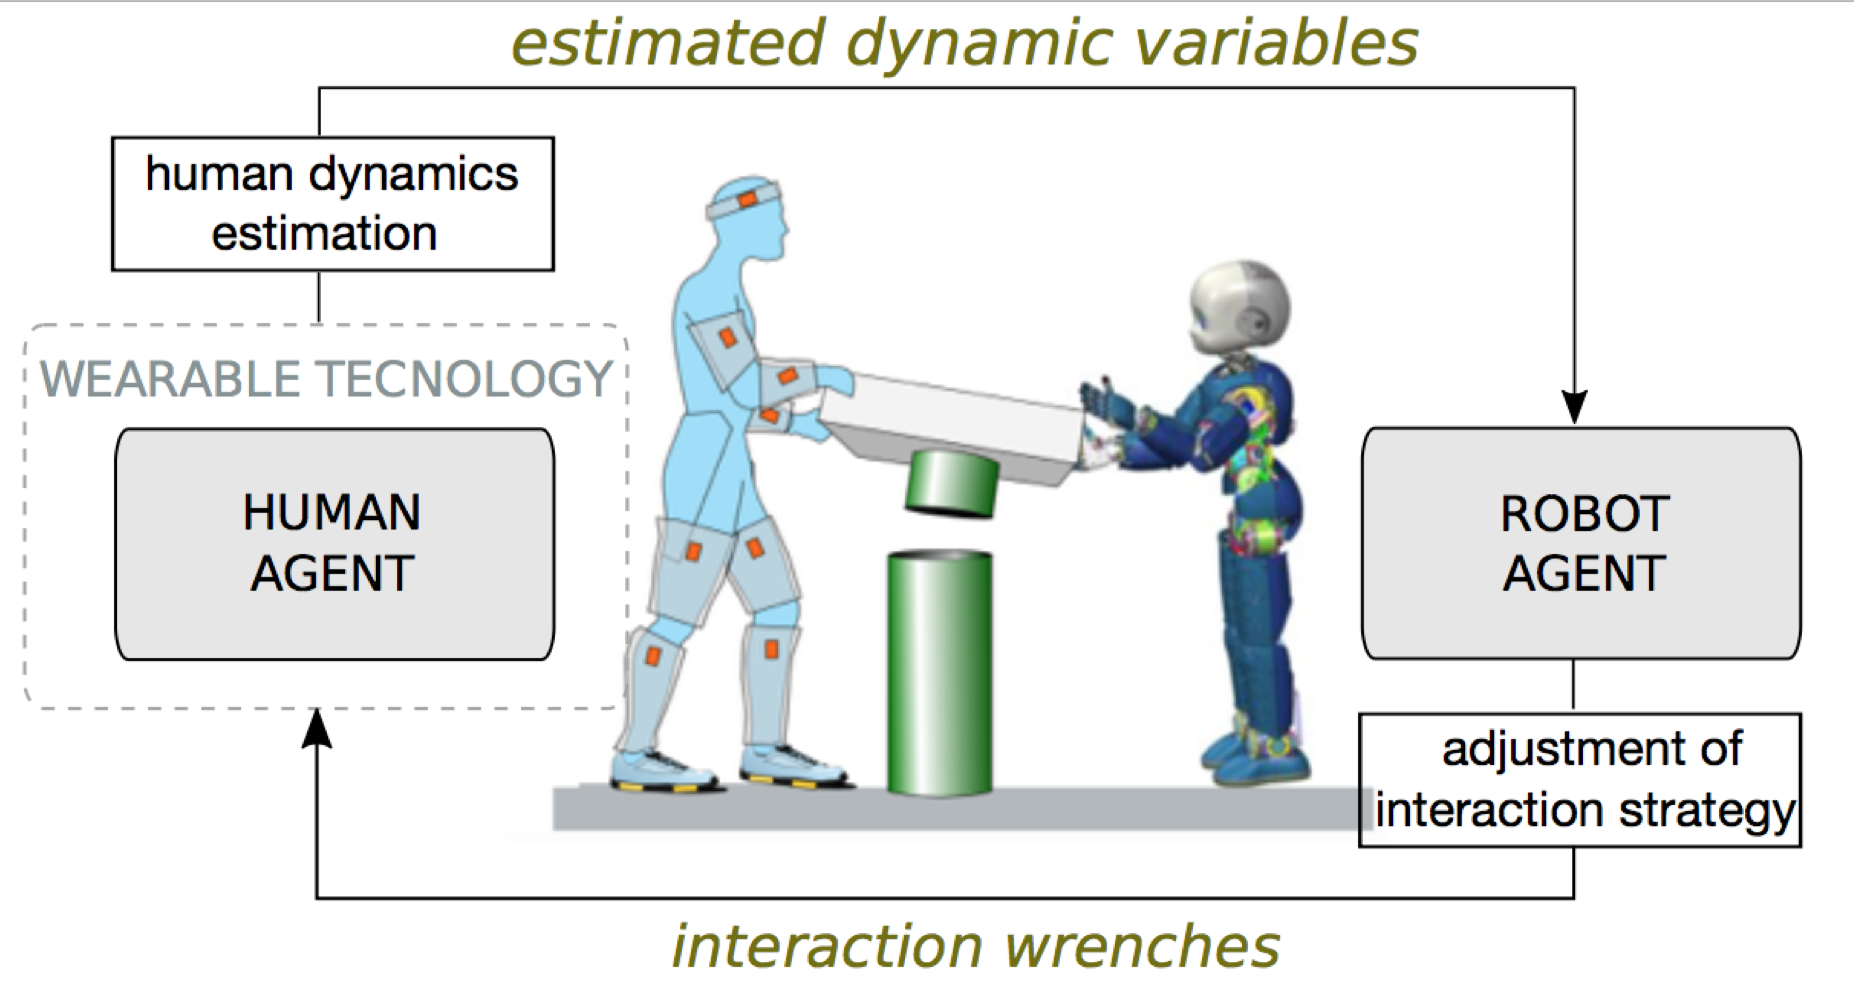
\includegraphics[width=1\columnwidth]{figs/schemeFramework}
  \caption{An example of pHRI scenario: the human agent is provided with a wearable 
  technology and an estimation algorithm allows to retrieve information about his dynamics. 
  By properly embedding estimations in the control loop of the robot, the 
  intentional collaboration may be enhanced.}
  \label{fig:figs_schemeFrameworkLoop}
\end{figure}
%!TEX root = ../template.tex

\section{Background}
%
The aim of this Section is to provide a rapid fast-forward of what is the current
 direction of the scientific community on this topic.  Most of the
  studies on the pHRI take inspiration from the intrinsic behaviour of the human nature:
   the \emph{mutual adaptive nature} that automatically occurs when two
    humans are cooperating together to accomplish a common task.  
	\\
	\indent
To this purpose, the importance of understanding human dynamics goes without saying and it is 
a crucial aspect of current state-of-the-art studies. Since humans
 move by minimizing jerk trajectories \cite{Flash1985},
 a method based on the minimum jerk model is used as a suitable approximation 
 for estimating the human partner motions in \cite{Maeda2001}. Here the attempt is that of
  incorporating human
  characteristics in the control strategy of the robot. The weakness in  this type of approach,
   however, lies in the pre-determination of the task and in the role that the robot has to
    play in the task execution.
   Furthermore, the minimum jerk model reliability decreases considerably if the human partner
    decides to apply non-scheduled trajectory changes during the task \cite{Miossec2009}.
	  Another route for pHRI is the \emph{imitation learning} approach, 
	  where the movements of two 
	 human actors are typically retrieved with motion capture techniques, clustered in motion
	  database (\cite{Guerra2011}, \cite{Kuehne2011}, \cite{Wojtusch2015}) and then used to 
	 learn the interaction skills (\cite{Amor2014}, \cite{Tamim2014}, \cite{Tamim2016}).
%
%%%%%%%%%%%%%%%%%%%%%%%%%%%%%%%%%%%%%%%%%%%%%%%%%%%%%%%%%%%%%%%%%%%%%%%%%%%%%%%%%%%%%%%%%%%%%%%%
\subsection{Problem statement}
Unlike the current leaning, we want to pay more attention on the key role that 
a proper sensing technology for human beings together with dynamics estimation algorithms
  may offer for retrieving whole-body motions and interaction forces. 
 More in detail, our work will be based on the formalism adopted for humanoid robots by 
 making the assumption of modelling the human body as a articulated rigid multi-body system. 
The advantage of this choice is evident since it allows to handle both systems
with the same mathematical tools. In this domain, the application of the Euler-Poincar\'{e} 
formalism \cite{Marsden2010} leads to three sets of equations describing:
    $i)$ the motion of the robot,
	$ii)$ the motion characterizing the human,
	$iii)$ the linking equations characterizing the contacts between human and robot. 
%
\begin{eqnarray*}
\label{robot}
i) \hspace{0.6cm} 
\bm {\mathrm{M}}(\bm {{q}}) \dot{\bm{v}} + \bm {\mathrm{C}}(\bm {{q}},
 \bm{v})
\bm{v} + \bm {\mathrm{G}}(\bm {{q}}) = \begin{bmatrix} \bm 0 \\ {\bm \tau}
 \end{bmatrix} + \bm {\mathrm{J}}^\top(\bm {{q}}) \bm{\mathrm{f}}
\end{eqnarray*}
%
\begin{eqnarray*}
\label{human}
ii) \hspace{0.6cm}
\mathbb{M}(\bar{\bm q}) \dot{\bar{\bm v}} + \mathbb{C}(\bar{\bm q}, \bar{\bm v})
\bar{\bm v} + \mathbb{G}(\bar{\bm q}) = \begin{bmatrix} \bm 0 \\ {\bm \tau} \end{bmatrix}
+ \mathbb{J}^\top(\bar{\bm q}) \bm{\mathrm{f}}
\end{eqnarray*}
%
\begin{eqnarray*}
\label{linking}
iii) \hspace{0.4cm}
\begin{bmatrix} \bm {\mathrm{J}}(\bm {{q}}) & ~\mathbb{J}(\bar{\bm q}) \end{bmatrix}
	\begin{bmatrix} \dot{\bm{v}} \\ \dot{\bar{\bm v}} \end{bmatrix} +
		\begin{bmatrix} \bm {\dot{\mathrm{J}}}(\bm {{q}}) & 
			~\dot{\mathbb{J}}(\bar{\bm q})
		 \end{bmatrix}
			\begin{bmatrix}{\bm{v}} \\ {\bar{\bm v}} \end{bmatrix} = \bm 0
\end{eqnarray*}
% \begin{eqnarray*}
% \label{linking}
% iii) \hspace{1.7cm} \mathbb{L}(
% \bm{{q}},
% \bar{\bm q},
% \bm{\bm v},
% \bar{\bm v},
% \dot{\bm v},
% \dot{\bar{\bm v}},
%  ) = \bm 0.
% \end{eqnarray*}
%
\indent
Equations $i)$ and $ii)$ are floating base system representations of the
dynamics of the robot and  human models, respectively. 
Vectors $\bm {{q}}$ and $\bar{\bm q}$ represent the configuration space (i.e. the position and orientation of a chosen frame, called base frame, and the joints configuration) of the two systems. The velocity is represented by $\bm{v}$
 and $\bar{\bm v}$ for robot and human systems, respectively.
 The matrices $\mathrm{M}$,
  $\mathrm{C}$, $\mathrm{G}$ and $\mathbb{M}$, $\mathbb{C}$, $\mathbb{G}$ denote the 
  mass matrix, Coriolis matrix and the gravity bias term for the robot and the human 
  systems, respectively.  
   The forces the two systems
  exchange are denoted by $\bm{\mathrm{f}}$, which owns a proper dimension depending on the
  number of wrenches\footnote{As an abuse of notation, we define as wrench a quantity that is
   not the dual of a twist but a vector $\in \mathbb R^{6}$ containing both the forces and 
   the related moments.} exchanged during the interaction task\footnote{For the sake of simplicity,
  we omitted the forces the two systems exchange with the external environment 
  (i.e., the ground) from the 
  formulation of $i)$ and $ii)$. As a straightforward consequence, the linking
   equations between each system with the external environment are not considered.}. 
  The Jacobians associated with the forces $\bm{\mathrm{f}}$ are denoted by
   $\bm {\mathrm{J}}(\bm{\mathrm{q}}) $ and $\mathbb{J}(\bar{\bm q})$.  
   In $iii)$ we make the assumption of rigid contacts between the two systems.
%!TEX root = ../template.tex

\section{Human Body Modelling}

We propose a human body reference model as an articulated multi-body skeleton with rigid
 bodies connected by 3 Degrees-of-Freedom (DoF) joints. Kinematic and dynamic properties 
 are defined as follows.
%
%%%%%%%%%%%%%%%%%%%%%%%%%%%%%%%%%%%%%%%%%%%%%%%%%%%%%%%%%%%%%%%%%%%%%%%%%%%%%%%%%%%%%%%%%%%%%%%%
\subsection{Kinematic properties}
Inspired by the biomechanical model developed for the Xsens MVN motion capture system
 \cite{Roetenberg2009} shown in Fig. \ref{fig:human_models}b, our model consists of a set of 
 23 rigid bodies with simple geometric
  shapes (parallelepiped, cylinder, sphere).  The origin of each link is located at 
  the parent joint origin, (i.e., the joint that connects the link to its
  parent). Figure \ref{fig:figs_human_JointLink}b shows  links and joints of the model.  
  The dimension of 
   each link is estimated by using data coming from motion capture acquisition.
%
\begin{figure}
  \centering
    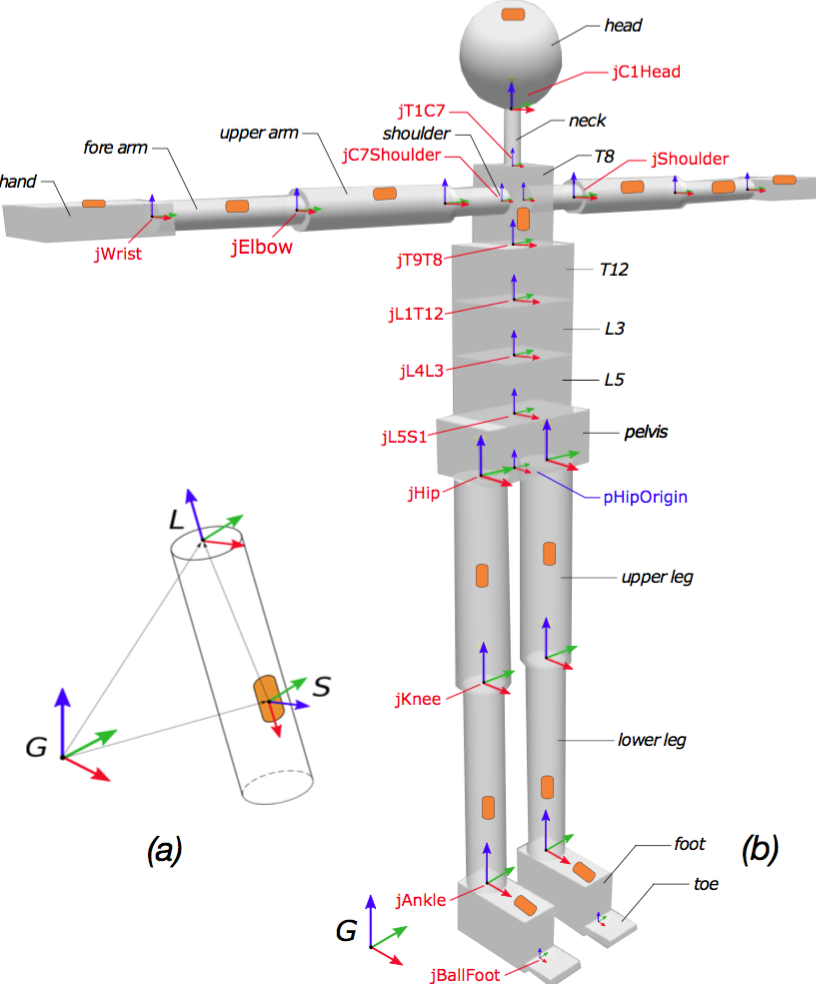
\includegraphics[width=1\columnwidth]{figs/human_JointLink}
\caption[Caption for LOF]{(a) Sensor attached to a generic link. 
(b) Human body reference model with labels for links and joints 
and with sensors distributed in the Xsens suit.  
 Reference frames are also shown\footnotemark.}
  \label{fig:figs_human_JointLink}
\end{figure}
%
\footnotetext{The RGB (Red-Green-Blue) convention for
${x}$-${y}$-${z}$ axes is adopted throughout the paper.}
%
%%%%%%%%%%%%%%%%%%%%%%%%%%%%%%%%%%%%%%%%%%%%%%%%%%%%%%%%%%%%%%%%%%%%%%%%%%%%%%%%%%%%%%%%%%%%%%%%
\subsection{Dynamic properties}
The dynamic properties, such as center of mass and inertia tensor for each link, are not
 embedded in the Xsens output data since they are usually computed in a post-processing phase.
   Since our aim is to have a real-time estimation for the human dynamic variables,
    the knowledge of
    dynamic properties during the acquisition phase is mandatory \cite{Drillis1964}.  Since it is impractical to retrieve these quantities in-vivo for humans, we relied on the
	 available anthropometric data in literature (\cite{Winter1990}, \cite{Herman2007})
	  starting from the total body mass of the
 subject, under the assumptions of geometric approximation and of homogeneous density for
  the rigid bodies (\cite{Hanavan1964}, \cite{Yeadon1990}).  
 %  
%%%%%%%%%%%%%%%%%%%%%%%%%%%%%%%%%%%%%%%%%%%%%%%%%%%%%%%%%%%%%%%%%%%%%%%%%%%%%%%%%%%%%%%%%%%%%%%%
%  \subsection{Sensor position}
% In order to build the model, the information of the position of the sensors for each link is
%  needed. Since it is not provided by Xsens, we exploited the linear acceleration $\bm a$ and
%   the angular velocity $\bm \omega$ measured by sensors in the following way:
%
% \begin{eqnarray} \label{eq:sensorPosEq} \nonumber
% {}^{S} \bm a_{S} &=& {}^{S} \bm R_G \Big( {}^{G} \bm a_{S} - {}^{G} \bm a_g \Big) =\\\nonumber
%                  &=& {}^{S} \bm R_G \Big[ {}^{G} \bm a_{L} + {}^{G} \bm{\dot \omega}_{L}
% 				     \times {}^{G} \bm R_{L} {}^{L} \bm p_{S, L}+\\
%                 &{}& {}^{G} \bm \omega_{L} \times \Big( {}^{G} \bm \omega_{L} \times
% 				     {}^{G} \bm R_{L} {}^{L} \bm p_{S, L}\Big) - {}^{G} \bm a_g \Big],
% \end{eqnarray}
% where $S$ is the frame of the sensor and $L$ is the frame related to the link on which it is
% attached (as in Fig. \ref{fig:figs_human_JointLink}a). By exploiting \eqref{eq:sensorPosEq}
% it is possible to retrieve the position of sensor on the link in
% the link frame ${}^{L} \bm p_{S, L}$.
%!TEX root = ../template.tex

\section{Probabilistic Sensor Fusion Algorithm}
%
In this Section we briefly recall the probabilistic method for estimating dynamic variables of
 an articulated mechanical system by exploiting the so-called sensor fusion information,
  already presented
  in our previous work (the reader should refer to \cite{LatellaSensors2016} for a more thorough
   presentation).
\\
\indent
From a theoretical point of view, we describe our model
 as a mechanical system represented by an oriented kinematic tree with $N_B$ moving links and
  $n$-DoFs.  Note that $n=n_1+...+n_{N_B}$ is the total number of DoFs of the system.  The
   generic $i$-th link  and its parent are coupled with a joint $i$ following 
  the topological Denavit-Hartenberg convention for joint numbering \cite{Denavit1955}.
We are interested in computing an estimation of a vector of \emph{dynamics variables} $\bm d$ defined as:
%
\begin{subequations} \label{eq:dynvec} 
	\begin{eqnarray*} 
    	\bm d &=& \begin{bmatrix} \bm d_{1}^\top & \bm
    	d_{2}^\top & \hdots & \bm d_{N_B}^\top \end{bmatrix}^\top 
    	\in \mathbb R^{24N_B+2n},\\
    \bm d_i &=& \begin{bmatrix} \bm
	a_{i}^\top &{\bm f_{i}^B}^\top & \bm f_{i}^\top & \bm \tau_{i} 
	& {\bm f_{i}^x}^\top & \ddot {\bm{q}}_{i} \end{bmatrix}^\top \in
	\mathbb R^{24+2n_i},
	\end{eqnarray*} 
\end{subequations}
%
where $\bm a_i$ is the $i$-th body spatial acceleration, $\bm {f_i}^B$ is the net
 wrench, $\bm f_i$ is the internal wrench exchanged from the parent link to the $i$-th link, 
 $\bm \tau_i \in \mathbb R^{n_i}$ is the torque at the joint, $\bm {f_i}^x$ is the external
  wrench applied by the environment to the link and $ \ddot{\bm q}_i  \in \mathbb R^{n_i}$ is
   the joint acceleration. The system can interact with the surrounding environment, and the
    result of this interaction is reflected in the presence of the external wrenches 
	$\bm {f_i}^x$.
	\\
	\indent
The dynamics of the mechanical system\footnote{We consider here the fixed base system
 configuration.} can be obtained from the application of the Newton-Euler
 equations\footnote{It is worth to notice that here we prefer to adopt the Newton-Euler
  formalism as an equivalent representation of the system dynamics. More details about 
  this choice in Section 3.3 of \cite{LatellaSensors2016}.} \cite{Featherstone2008}.  
  It is possible to rearrange these equations
  into a matrix form thus obtaining the following linear system of equations in the variable
    $\bm d$:
%
\begin{equation} \label{eq:matRNEA} 
\bm D(\bm q, \dot {\bm q}) \bm d + \bm b_D 
(\bm q,\bm {\dot q})= \bm 0,
\end{equation}
where the matrix $\bm D \in \mathbb R^{(18 N_B+n) \times \bm d}$  and the bias vector
$\bm b_D \in \mathbb R^{18 N_B+n}$.  We now consider the presence of $N_S$ measurements of dynamic quantities coming from different
 sensors (e.g. accelerometers, force/torque sensors) and we denote with $\bm y \in \mathbb
  R^{N_S}$ the vector containing all the measurements.  The dynamic variables and the values
   measured by the sensors can be related by the following set of equations:
%
\begin{equation} \label{eq:measRNEA} 
\bm Y(\bm q, \dot {\bm q}) \bm d + \bm b_Y (\bm q,\bm {\dot q})= \bm y,
\end{equation}
where $\bm Y \in \mathbb R^{N_S \times \bm d}$ and $\bm b_Y \in \mathbb R^{N_S}$.  By stacking
 together \eqref{eq:matRNEA} and \eqref{eq:measRNEA} we obtain a linear system of
  equations in the variable $\bm d$:
%
\begin{eqnarray} \label{eq:systemEq} 
\begin{bmatrix}
\bm Y(\bm q,\dot {\bm q}) \\ \bm D(\bm q, \dot {\bm q}) \\
 \end{bmatrix}\bm d + \begin{bmatrix} \bm b_Y(\bm q, \dot {\bm q})
\\ \bm b_D(\bm q, \dot {\bm q}) \end{bmatrix} = \begin{bmatrix} \bm y\\
 \bm 0 \end{bmatrix}. 
\end{eqnarray}
%
\indent
Equation \eqref{eq:systemEq} describes, in general, an overdetermined linear system of
 equations.  The bottom part, corresponding to \eqref{eq:matRNEA} represents the
  Newton-Euler equations, while the upper part contains the information coming from the,
   possibly noisy or redundant, sensors.
It is possible to compute the whole-body dynamics estimation
by solving the system in \eqref{eq:systemEq} for $\bm d$.  One possible approach is to solve \eqref{eq:systemEq} in the
 least-square sense, by using a Moore-Penrose pseudoinverse or a weighted pseudo-inverse.  
 
 In the following we perform a different choice.  
  We frame the estimation of $\bm d$ given the knowledge of $\bm y$ and prior information 
  about the model and the sensors in a Gaussian domain by
   means of a \emph{Maximum-a-Posteriori} (MAP) estimator\footnote{The benefits of the MAP
    estimator choice are explained in Section 4 of \cite{LatellaSensors2016}.} such that
%
\begin{equation*} 
\bm d_{\mbox\footnotesize{MAP}}=\arg \max_{\bm d} p(\bm d| \bm y) .
\end{equation*}
Since in this framework probability distributions are associated to both the measurements
 and the model, it suffices to
 compute the expected value and the covariance matrix of $\bm d$ given $\bm y$, i.e.
%
\begin{subequations}\label{eq:d_y} 
	\begin{eqnarray}\label{eq:d_ySigma} 
	 \bm {\Sigma}_{d|y}& = & \left(\bar{\bm {\Sigma}}_D^{-1}+ \bm Y^\top \bm 
	 {\Sigma}_{y}^{-1} \bm Y \right)^{-1},\\ \label{eq:d_yMu} 
	 \bm {\mu}_{d|y} &= & \bm {\Sigma}_{d|y} \left[ \bm Y ^\top \bm {\Sigma}_{y}^{-1} 
	 (\bm y - \bm b_Y) + \bar{\bm {\Sigma}}_D^{-1} \bar {\bm {\mu}}_D \right],
    \end{eqnarray} 
\end{subequations}
%
where $\bar{\bm {\mu}}_D$ and $\bar{\bm {\Sigma}}_D$ are the mean and 
covariance of the probability distribution 
 ${p(\bm d) \sim \mathcal N \left(\bar  
{\bm {\mu}}_D, \bar {\bm {\Sigma}}_D\right)}$ of the model, respectively;
 $\bm {\Sigma}_{y}$ is the covariance 
matrix of the distribution ${p(\bm y)\sim\mathcal N \left({\bm {\mu}}_y, {\bm {\Sigma}}_y\right)}$ related to the measurements.
  In the Gaussian framework, \eqref{eq:d_yMu} 
corresponds to the estimation of $\bm d_{\mbox\footnotesize{MAP}}$.  
It is worth noting that the vector $\bm d$ contains, among the other dynamic variables, an estimate of the joint torque $\bm \tau$ for retrieving the inverse dynamics estimation.
%!TEX root = ../template.tex

\section{Experimental Design}
%
Data were collected at Istituto Italiano di Tecnologia (IIT), Genoa, Italy. The experimental
set-up encompasses the following different sensor modules: 
$j)$ a wearable suit for the motion tracking,
$jj)$ two standard force platforms to acquire the ground reaction wrenches, 
$jjj)$ the force/torque sensors of the robot arms. 
%
%%%%%%%%%%%%%%%%%%%%%%%%%%%%%%%%%%%%%%%%%%%%%%%%%%%%%%%%%%%%%%%%%%%%%%%%%%%%%%%%%%%%%%%%%%%%%%%%
\subsection{Human configuration}
Ten healthy adult subjects (7 female, 3 male) have been recruited in the experimental 
session, height (\unit{166,6\pm4,5}{\centi\meter}) and 
mass (\unit{61,14\pm5,76}{\kilo\gram}).
Each subject was provided of a written informative consent before starting the experiment. Kinematics
  data were acquired by using a full-body wearable lycra suit provided by Xsens Technologies.  
The wearable suit is composed of 17 wired trackers, (i.e., inertial sensor units-IMUs including an
 accelerometer, a gyroscope and a magnometer). The suit has signal transmitters that send
  measurements to the acquisition unit through a wireless receiver which collects data at a
   frequency of \unit{240}{\hertz}. The human subject performed the required
    task standing with the
   feet on two standard force platforms AMTI OR6 mounted on the ground, while interacting 
   with the robot.
	  Each platform acquired a wrench sample at a frequency of
	   \unit{1}{\kilo\hertz} by using AMTI acquisition units. 
%
\begin{figure}
  \centering
    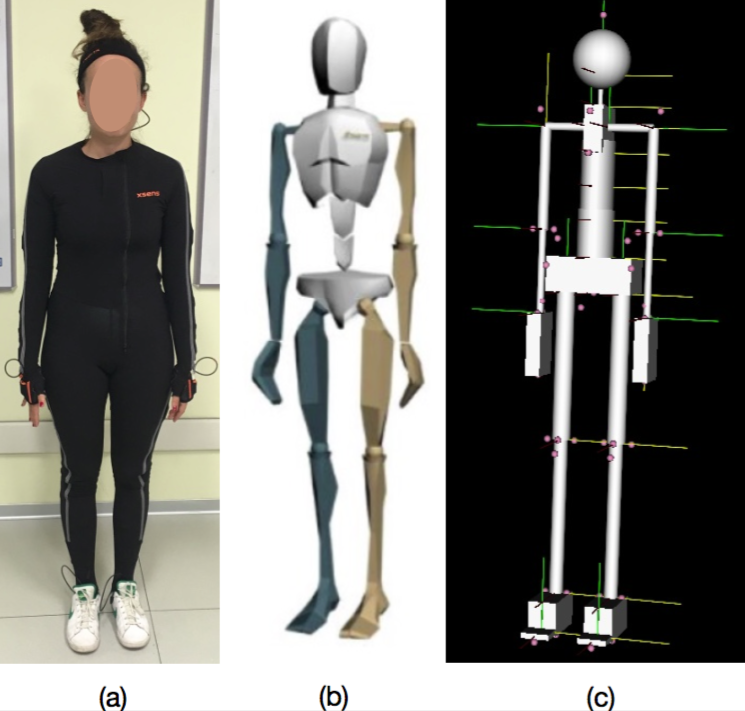
\includegraphics[width=0.9\columnwidth]{figs/humanModels}
  \caption{(a) Subject with the motion capture suit. (b) The Xsens MVN model. (c) Model reconstructed in OpenSim by using virtual markers from Xsens acquisition.}
 \label{fig:human_models}
\end{figure}
%
%%%%%%%%%%%%%%%%%%%%%%%%%%%%%%%%%%%%%%%%%%%%%%%%%%%%%%%%%%%%%%%%%%%%%%%%%%%%%%%%%%%%%%%%%%%%%%%%
\subsection{Robot configuration}
Experiments were conducted on the iCub \cite{Metta2010}, a full-body humanoid
robot (Fig. \ref{fig:iCub_couple}a) with 53-DoFs: 6 in the head, 16 in each arm, 3 in the
 torso and 6 in each leg. The iCub is endowed with whole-body distributed force/torque sensors,
  accelerometers, gyroscopes and tactile sensors. Specifically, the limbs are equipped with six
   force/torque sensors placed in the upper arms, in the upper legs and in the ankles 
   (Fig. \ref{fig:iCub_couple}b). Internal joint torques and external wrenches are estimated
    through an online whole-body estimation algorithm \cite{Nori2015icub}. Measurements for the
    wrenches exchanged between the robot and the human are obtained thanks to it.  Robot data
	 were collected at a frequency of \unit{100}{\hertz}.
%
\begin{figure}
  \centering
    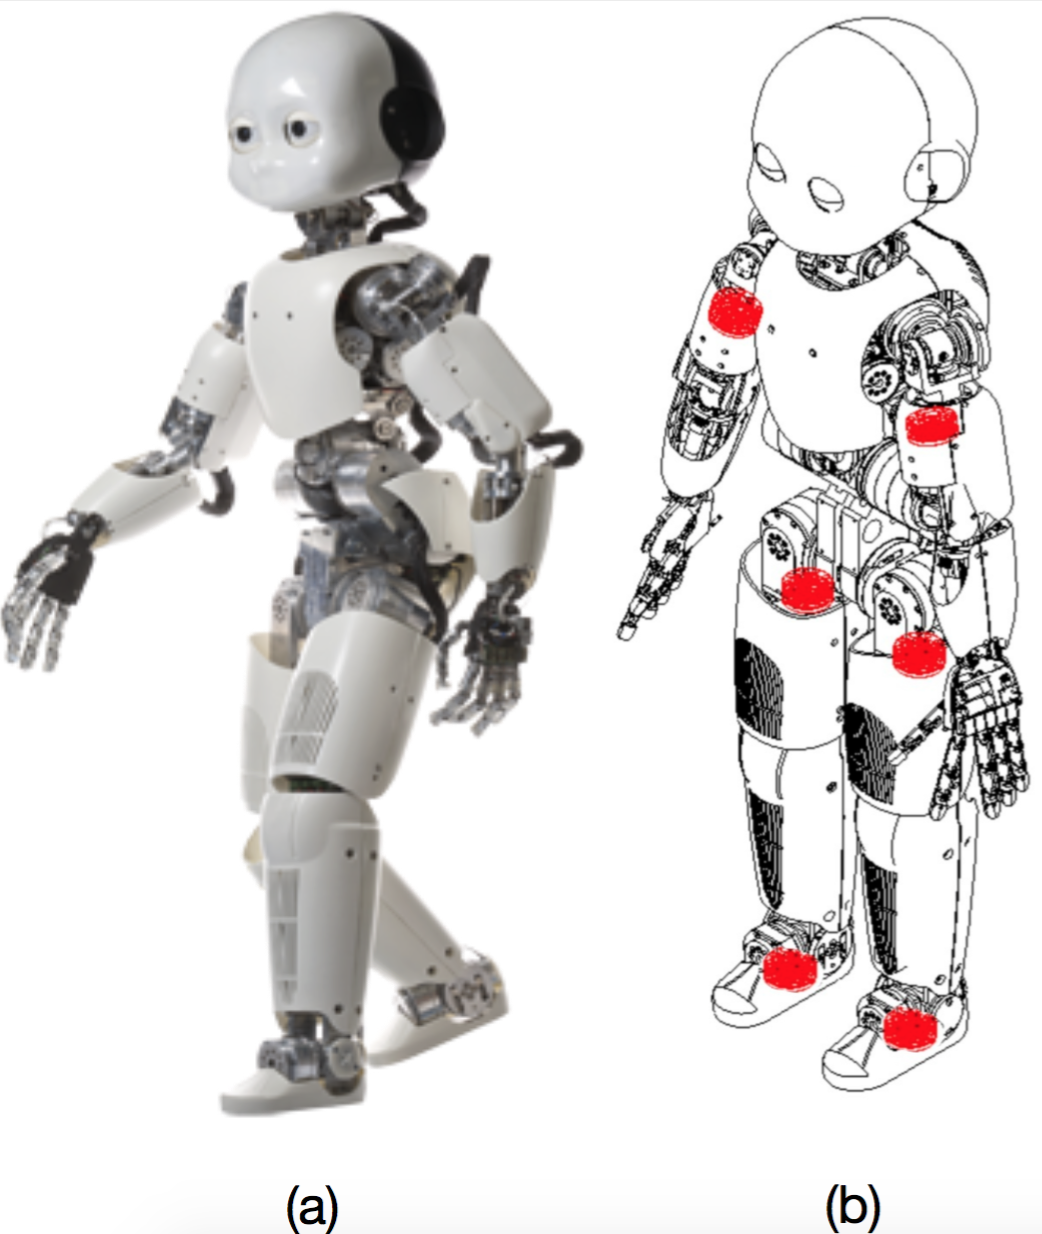
\includegraphics[width=0.75\columnwidth]{figs/iCub_couple}
  \caption{(a) The humanoid iCub. (b) Model of the iCub with the force/torque 
  sensors embedded in the limbs structure.}
  \label{fig:iCub_couple}
\end{figure}
%
%%%%%%%%%%%%%%%%%%%%%%%%%%%%%%%%%%%%%%%%%%%%%%%%%%%%%%%%%%%%%%%%%%%%%%%%%%%%%%%%%%%%%%%%%%%%%%%%
\subsection{Procedure protocol}
Each subject was asked to wear the suit (Fig. \ref{fig:human_models}a) and to stand on the 
two force plates by positioning each foot per platform. The robot 
  was located in front of the subject facing him at a known distance from the human foot
   location (as shown in Fig. \ref{fig:interaction_lateral&top}a). The mutual feet position was
    fixed for all the trials (Fig. \ref{fig:interaction_lateral&top}b).  
	The interaction implied that the human grasped and pushed down both robot arms 
	(Fig. \ref{fig:interaction_lateral&top}a) for those tasks that required the interaction.
	The subject performed:
	\begin{itemize}
		\item a bowing task ($BT$) without (Fig. \ref{fig:sequenceTask}a) and with
		 (Fig. \ref{fig:sequenceTask}b) the robot interaction;
		\item a squat task ($ST$) without (Fig. \ref{fig:sequenceTask}c) and with
		 (Fig. \ref{fig:sequenceTask}d) the robot.
		\end{itemize} 
All subjects had to perform five repetitions of the block composed of the above-mentioned
 tasks. In each block the order of tasks execution was randomized in order to make each 
trial as independent as possible among the blocks.
%
\begin{figure}[ht]
  \centering
    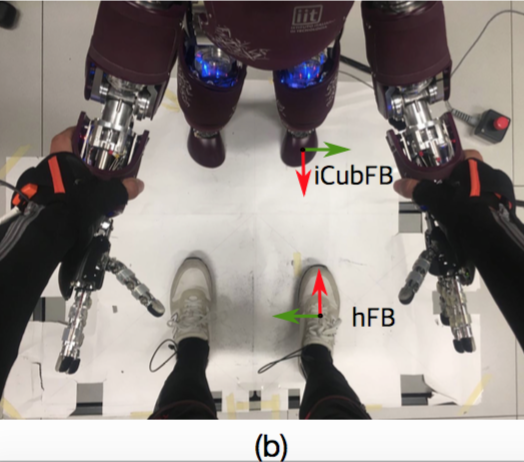
\includegraphics[width=6cm]{figs/interaction_lateralAndTop}
          \caption{(a)  Subject grasps and pushes down the robot arms.  The figure shows the
		  reference frames for the force/torque sensor of the robot (iCubFT), the robot fixed
		   base (iCubFB), the force plate (FP), the human fixed base (hFB), the human foot and
		    hand (hFOOT, hHAND) respectively. (b) Top view for the fixed feet position layout.}
			\label{fig:interaction_lateral&top}
\end{figure}
%
% \begin{figure}[h]
%   \centering
%    \begin{subfigure}[b]{0.5\columnwidth}
%       \includegraphics[width=\textwidth]{figs/interactionFrames.pdf}
%           \caption{}
%           \label{fig:figs_interactionFrames}
%   \end{subfigure}
%    \begin{subfigure}[b]{0.6\columnwidth}
%     \includegraphics[width=\textwidth]{figs/fixedTopView.pdf}
% 	\caption{}
%         \label{fig:fixedPositionTospView}
%    \end{subfigure}
%           \caption{(a)  Subject grasps and pushes down the robot arms.  The figure shows the
% 		  reference frames for the force/torque sensor of the robot (iCubFT), the robot fixed
% 		   base (iCubFB), the force plate (FP), the human fixed base (hFB), the human foot and
% 		    hand (hFOOT, hHAND) respectively. (b) Top view for the fixed feet position layout.}
% \end{figure}
%
\begin{figure*}[!ht]
  \centering
    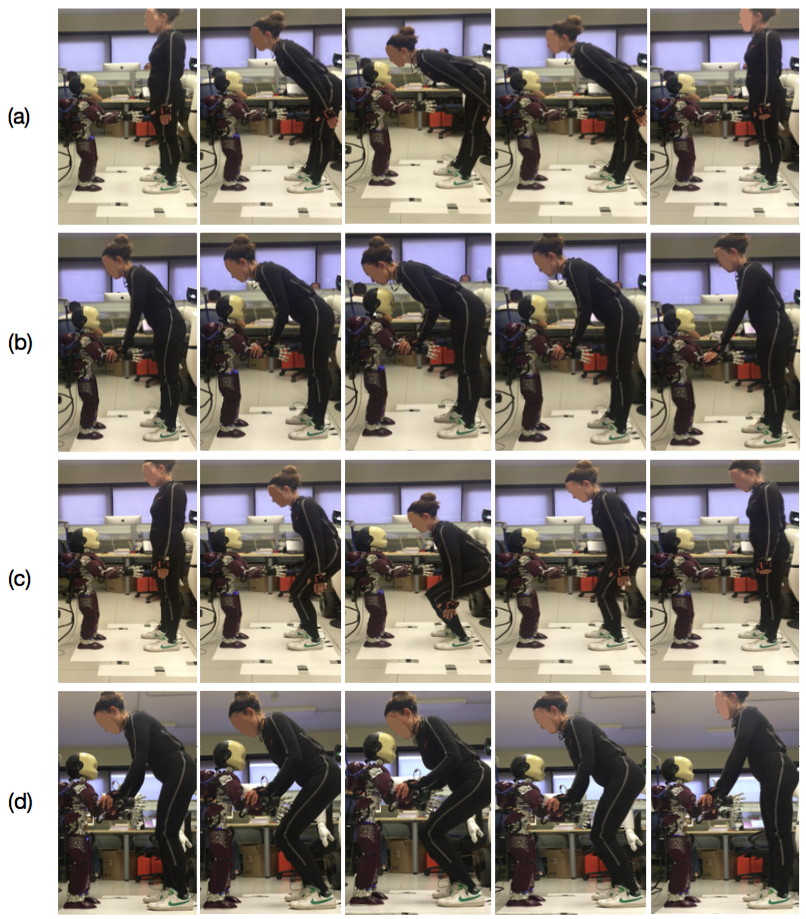
\includegraphics[width=0.75\textwidth]{figs/sequenceTask}
		  \caption{Subject performing: a $BT$ without (a) and with (b) the iCub,
		  a $ST$ without (c) and with (d) the iCub.}
			\label{fig:sequenceTask}
\end{figure*}
%
 % \begin{figure*}[h!]
 % 	 \centering
 % 	\begin{subfigure}[b]{0.7\textwidth}
 % 		\includegraphics[width=\textwidth]{figs/h_bowing.pdf}
 % 		\caption{}
 % 		\label{fig:h_bowing}
 % 	 \end{subfigure}
 % 	\begin{subfigure}[b]{0.7\textwidth}
 % 		\includegraphics[width=\textwidth]{figs/hri_bowing.pdf}
 % 		\caption{}
 % 		\label{fig:hri_bowing}
 % 	 \end{subfigure}
 % 	\begin{subfigure}[b]{0.7\textwidth}                                                                 \includegraphics[width=\textwidth]{figs/h_squat.pdf}
 % 		  	\caption{}
 % 		  	\label{fig:h_squat}
 % 	 \end{subfigure}
 %  	\begin{subfigure}[b]{0.7\textwidth}                                                                 \includegraphics[width=\textwidth]{figs/hri_squat.pdf}
 % 		  	\caption{}
 % 		  	\label{fig:hri_squat}
 %  	 \end{subfigure}
 %     \caption{Subject performing: a $BT$ without (a) and with (b) the iCub,
 % 	 a $ST$ without (c) and with (d) the iCub.}
 % \end{figure*}
%
%%%%%%%%%%%%%%%%%%%%%%%%%%%%%%%%%%%%%%%%%%%%%%%%%%%%%%%%%%%%%%%%%%%%%%%%%%%%%%%%%%%%%%%%%%%%%%%%
\subsection{Data processing}
Since the acquisition sampling rate was different among the sources, data are linearly
 interpolated in order to guarantee the synchronization. An overview of the framework is
  summarised in Fig. \ref{fig:figs_schemeAlgorithm}. Data coming from the force plates and from
   the robot (${\bm f^x}$) are considered as acquired from a particular class of net external
    wrench sensors. Linear acceleration $\bm a$ and angular velocity $\bm \omega$ for each
	 link are acquired by Xsens inertial sensors.
Xsens data are used as input for the OpenSim \cite{Delp2007} IK (Inverse Kinematics)
 toolbox that allowed to retrieve the joint angles $\bm q$ by matching 
 the marker positions of the OpenSim model (Fig. \ref{fig:human_models}c) and the virtual
 ones coming from Xsens data.
 Joint velocities $\bm {\dot q}$ and accelerations $\bm {\ddot q}$  are
    computed by using a weighted sum of windows of elements, with a third-order polynomial
	 Savitzky-Golay filtering. Also joint accelerations are considered as acquired from
	  a class of DoF acceleration sensors. In general, by considering as inputs data acquired
	   from all above-mentioned sensors and the state $(\bm q,\bm {\dot q})$, the MAP
	    estimator provides the estimation of $\bm d$ given $\bm y$.
%
% \begin{figure}[h]
%   \centering
%    \begin{subfigure}[b]{1\columnwidth}
%     \includegraphics[width=\textwidth] {figs/ExpSetUp.pdf}
%         \caption{}
%         \label{fig:devicesScheme}
% \end{subfigure}
%  \begin{subfigure}[b]{0.9\columnwidth}
%     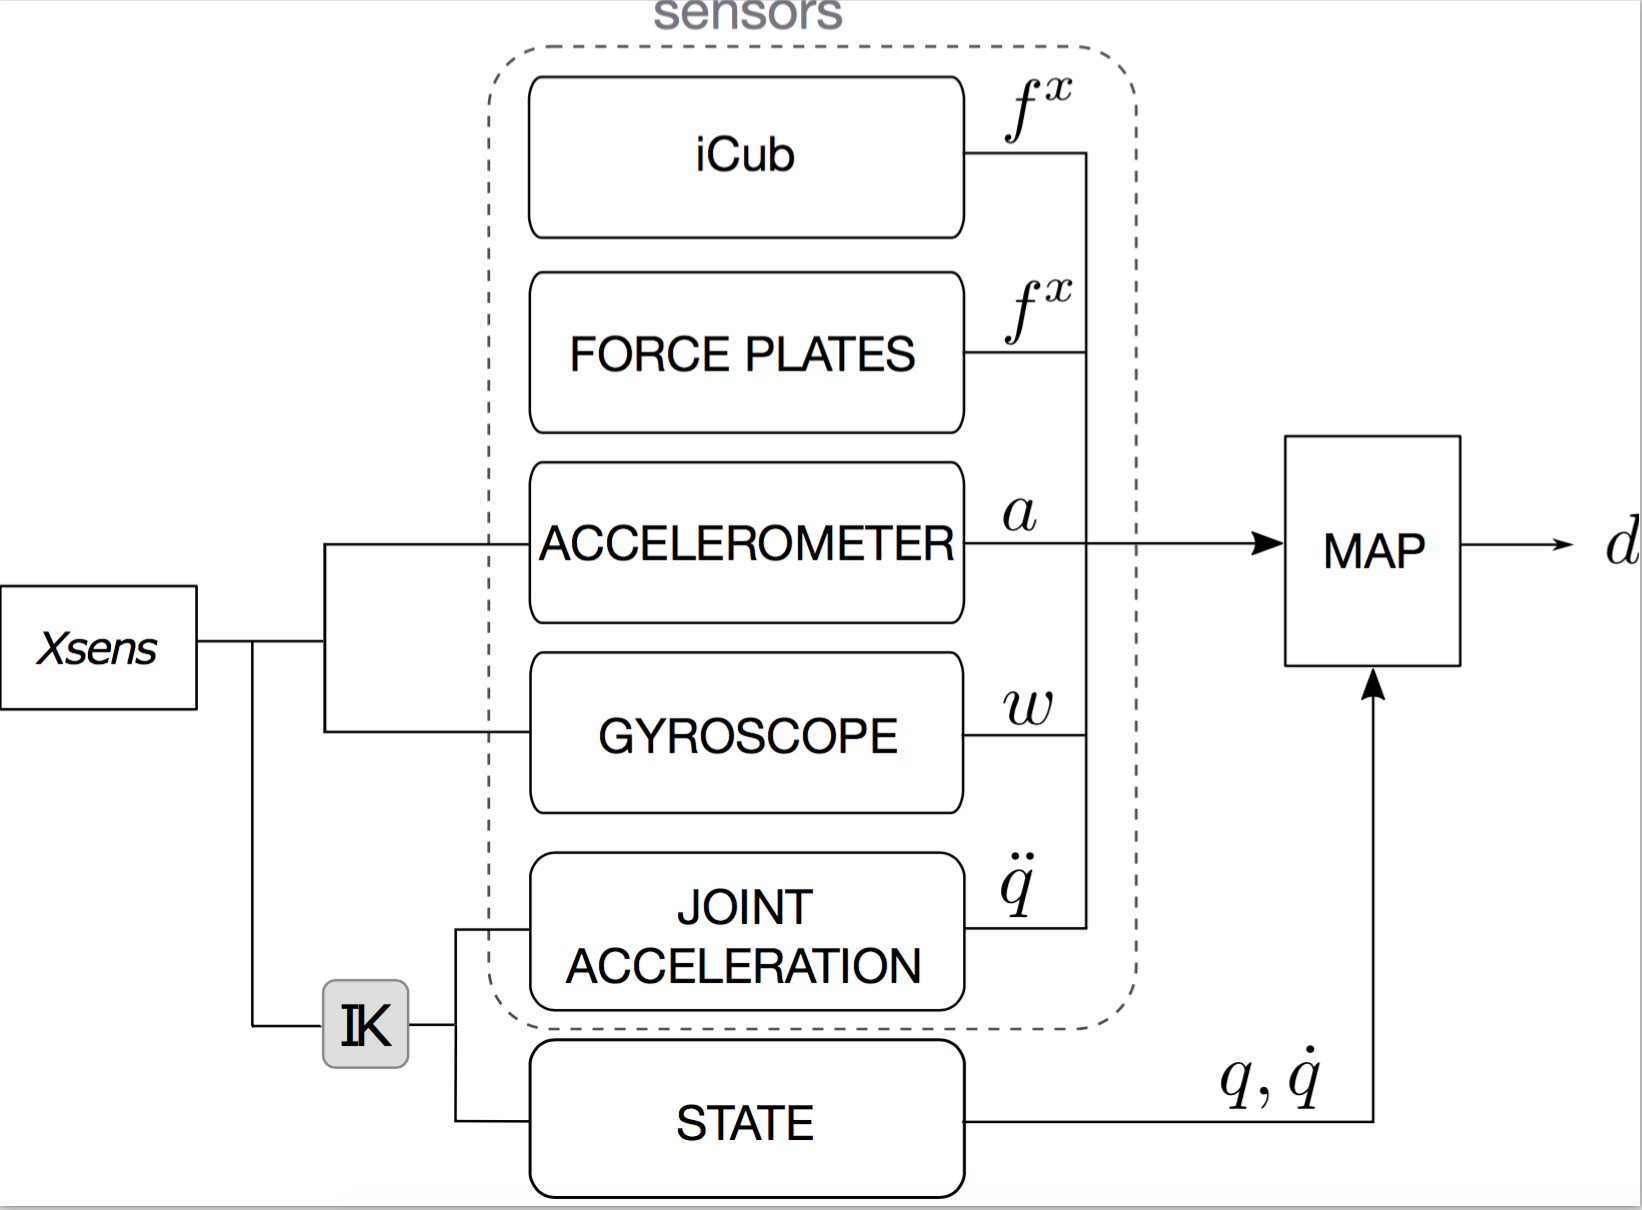
\includegraphics[width=\textwidth]{figs/schemeAlgorithm.pdf}
%         \caption{}
%         \label{fig:algorithmScheme}
% \end{subfigure}
%   \caption{(a) (b)xxx}
%   \label{fig:overview}
% \end{figure}

% \begin{figure}
% 	\centering
% 	  \def\svgwidth{0.9\columnwidth}
% 	  \import{figs/}{drawing.pdf_tex}
% \end{figure}
%
\begin{figure}
  \centering
    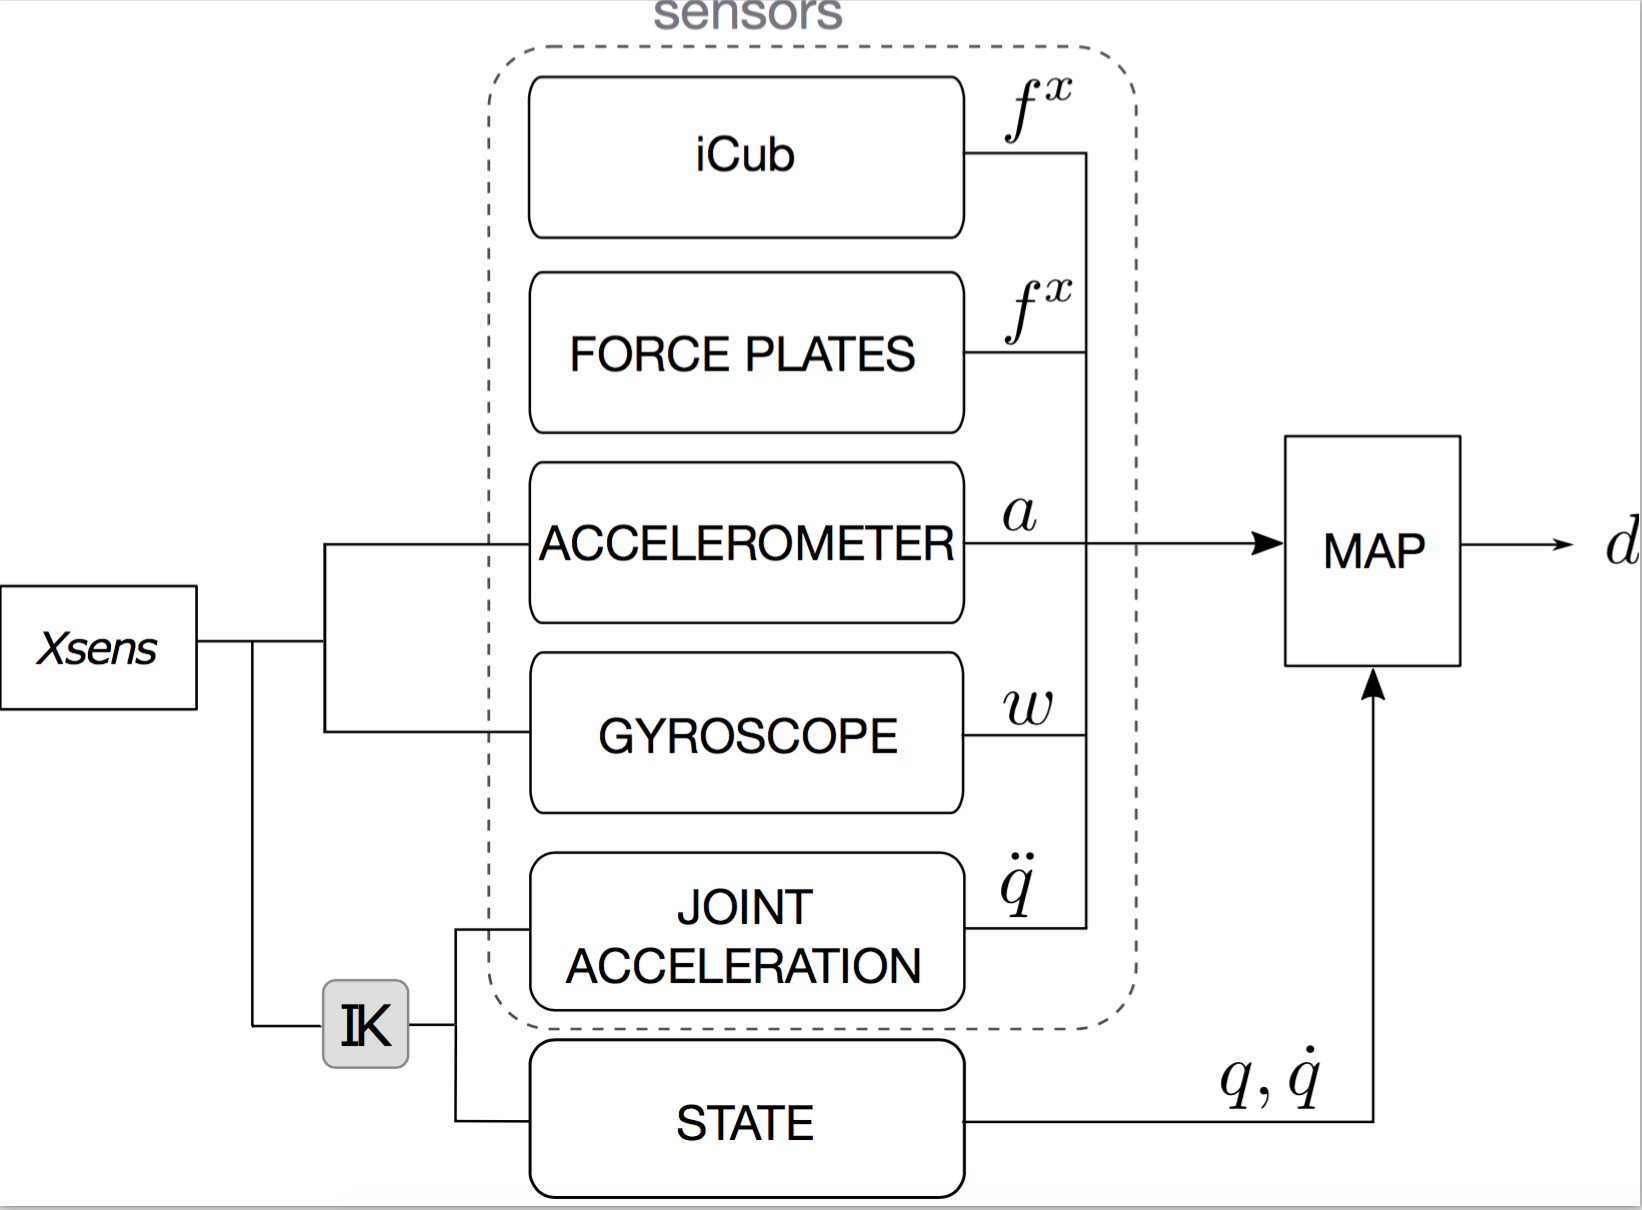
\includegraphics[width=1\columnwidth]{figs/schemeAlgorithm}
  \caption{Overview of the MAP estimation algorithm.} 
  \label{fig:figs_schemeAlgorithm}
\end{figure}
% %!TEX root =  ../D5.4.tex

\section{Experimental Results}
%
In this Section we discuss the evaluation procedure to prove the computation effectiveness of
 our estimation algorithm. The analysis was mainly performed on Matlab. 
 %and the related code 
%is freely available on Github\footnote{\texttt{https://github.com/claudia-lat/MAPest}}.
%
%%%%%%%%%%%%%%%%%%%%%%%%%%%%%%%%%%%%%%%%%%%%%%%%%%%%%%%%%%%%%%%%%%%%%%%%%%%%%%%%%%%%%%%%%%%%%%%%
\subsection{Torques estimation}
The core of the experiment consists in estimating the
 variable $\bm d$.  Among the variables contained in $\bm d$, the quantities of major 
 interest in our analysis are 
 the torques $\bm{\tau}$. We consider the internal
 torques developed along the $y$ axis in which the most significant angle variation is observed. 
In particular, we take into account the torque at the hip for $BT$ and the knee for $ST$. Since
 the torque estimation provides qualitatively a comparable result for both the two sides of 
 the human body, it is exhaustive to show only the torques associated to one side, e.g. the
  right one.
The value of the torque mostly depends on the kinematics and further on the 
inertial parameters of the subject and therefore, in order to compare torques across different subjects,
 it has to be normalized by considering the maximum and minimum values of each 
 subject's torque. 
Figures \ref{fig:figs_torqueRightHipBH}-\ref{fig:figs_torqueRightHipBRA} show the mean 
and the standard deviation of the right hip $\bm{\tau}$ estimation  without and 
with the interaction with the robot, respectively.  Figures \ref{fig:figs_torqueRightKneeSH}-\ref{fig:figs_torqueRightKneeSR} show the same 
quantities for the torques at the right knee in a $ST$ task.
%
% \begin{figure}[h!]
%   \centering
%    \begin{subfigure}[b]{0.49\columnwidth}
%       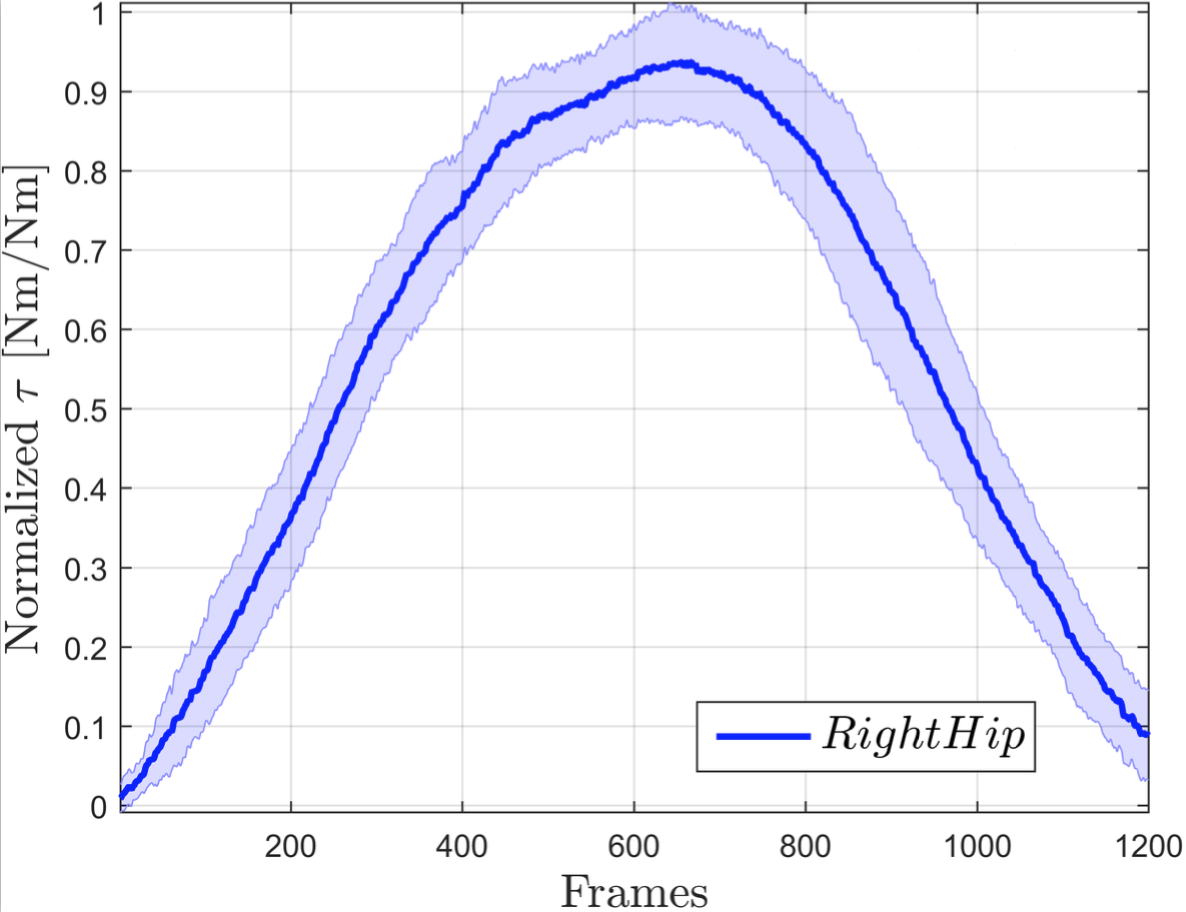
\includegraphics[width=\textwidth]{figs/torqueRightHipBH.pdf}
%           \caption{}
%           \label{fig:figs_torqueRightHipBH}
%   \end{subfigure}
%    \begin{subfigure}[b]{0.49\columnwidth}
%     \includegraphics[width=\textwidth]{figs/torqueRightHipBRA.pdf}
% 	\caption{}
%         \label{fig:figs_torqueRightHipBRA}
%    \end{subfigure}
%    \begin{subfigure}[b]{0.49\columnwidth}
%     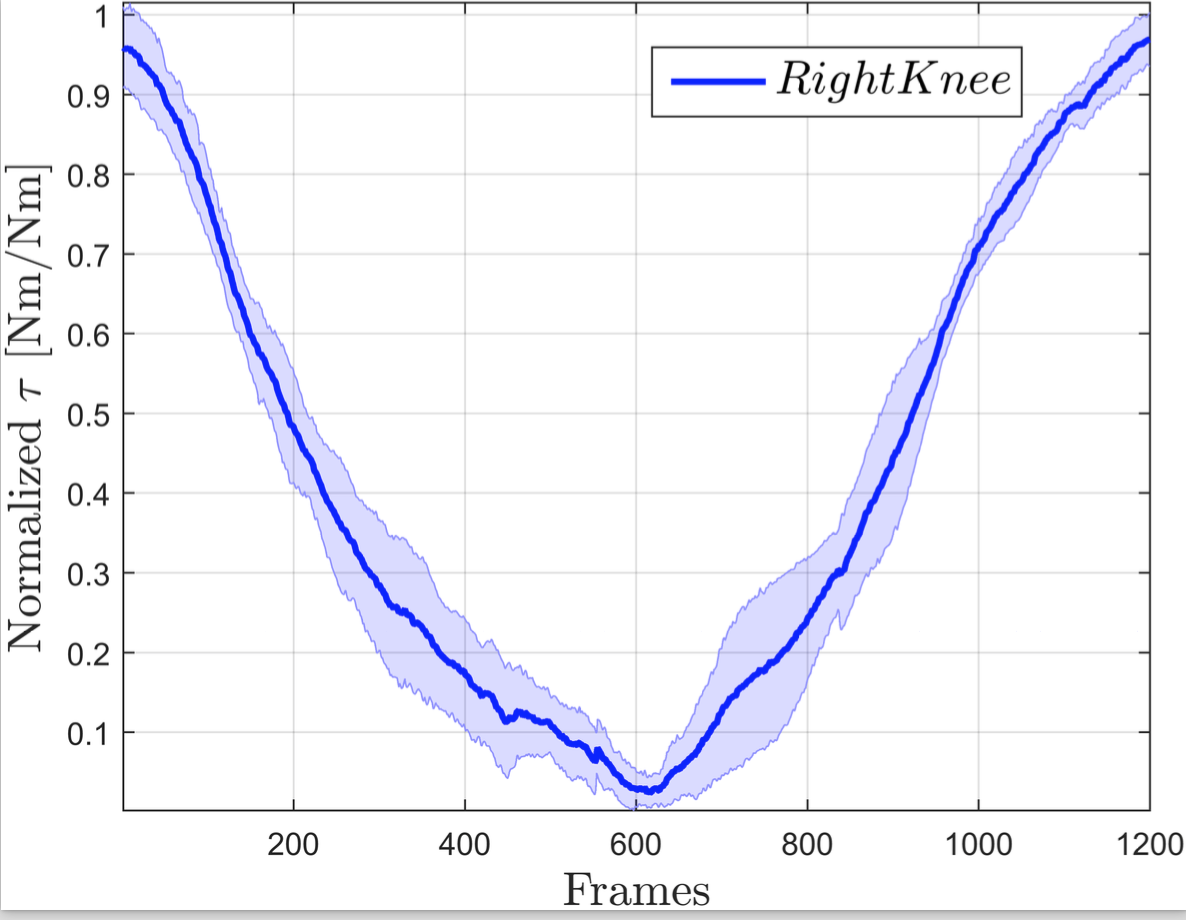
\includegraphics[width=\textwidth]{figs/torqueRightKneeSH.pdf}
% 	\caption{}
%         \label{fig:figs_torqueRightKneeSH}
%    \end{subfigure}
%    \begin{subfigure}[b]{0.49\columnwidth}
%     \includegraphics[width=\textwidth]{figs/torqueRightKneeSR.pdf}
% 	\caption{}
%         \label{fig:figs_torqueRightKneeSR}
%    \end{subfigure}
%           \caption{\emph{Inter-subjects analysis}: normalised right hip torques of 10 subjects
% 		  (mean and standard deviation) for BT without (a) and with (b) robot, for ST without
% 		   (c) and with (d) robot.}
% \end{figure}
%
 \begin{figure*}[!ht]
	 \centering
	%\begin{subfigure}[b]{0.48\textwidth}
		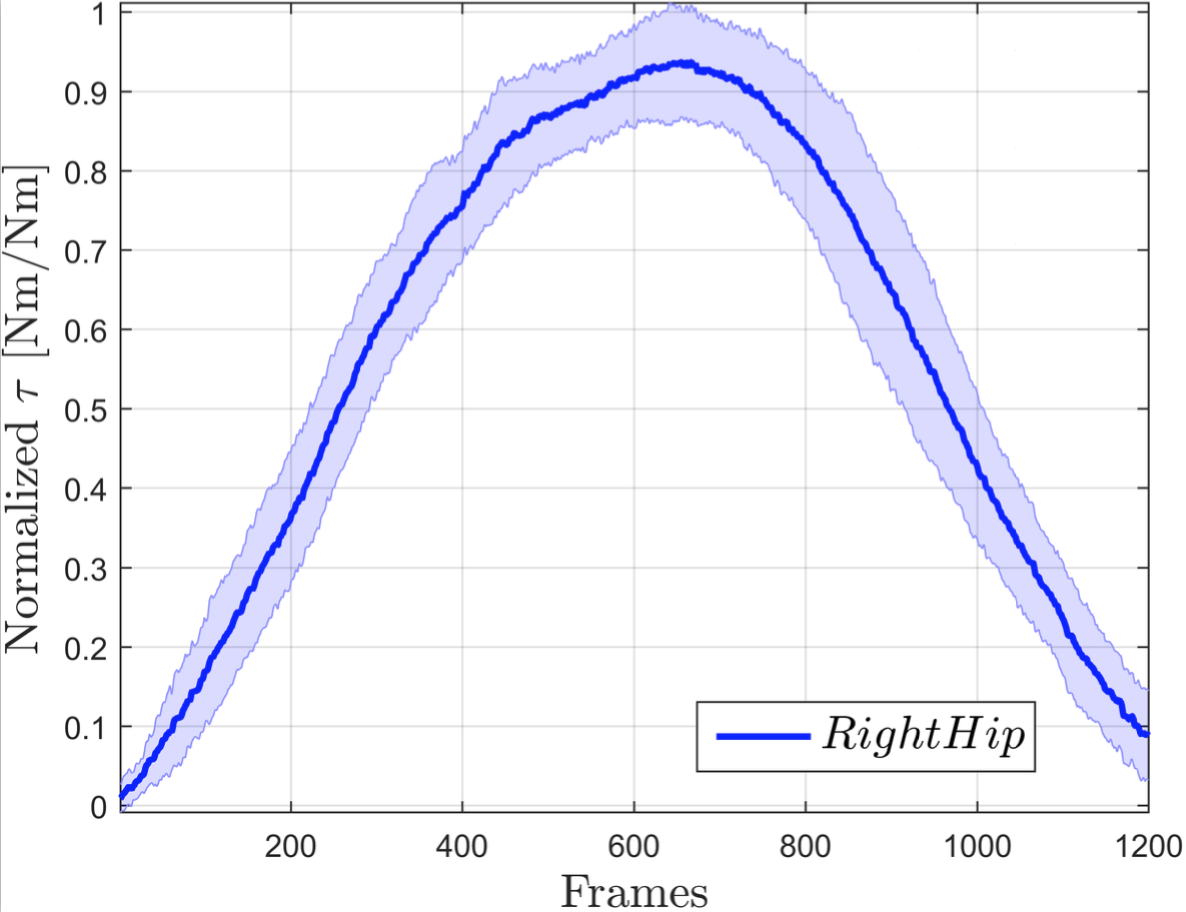
\includegraphics[width=0.48\textwidth]{figs/torqueRightHipBH}
	%	\caption{}
	%	\label{fig:figs_torqueRightHipBH}
	% \end{subfigure}
 %	\begin{subfigure}[b]{0.48\textwidth}
 		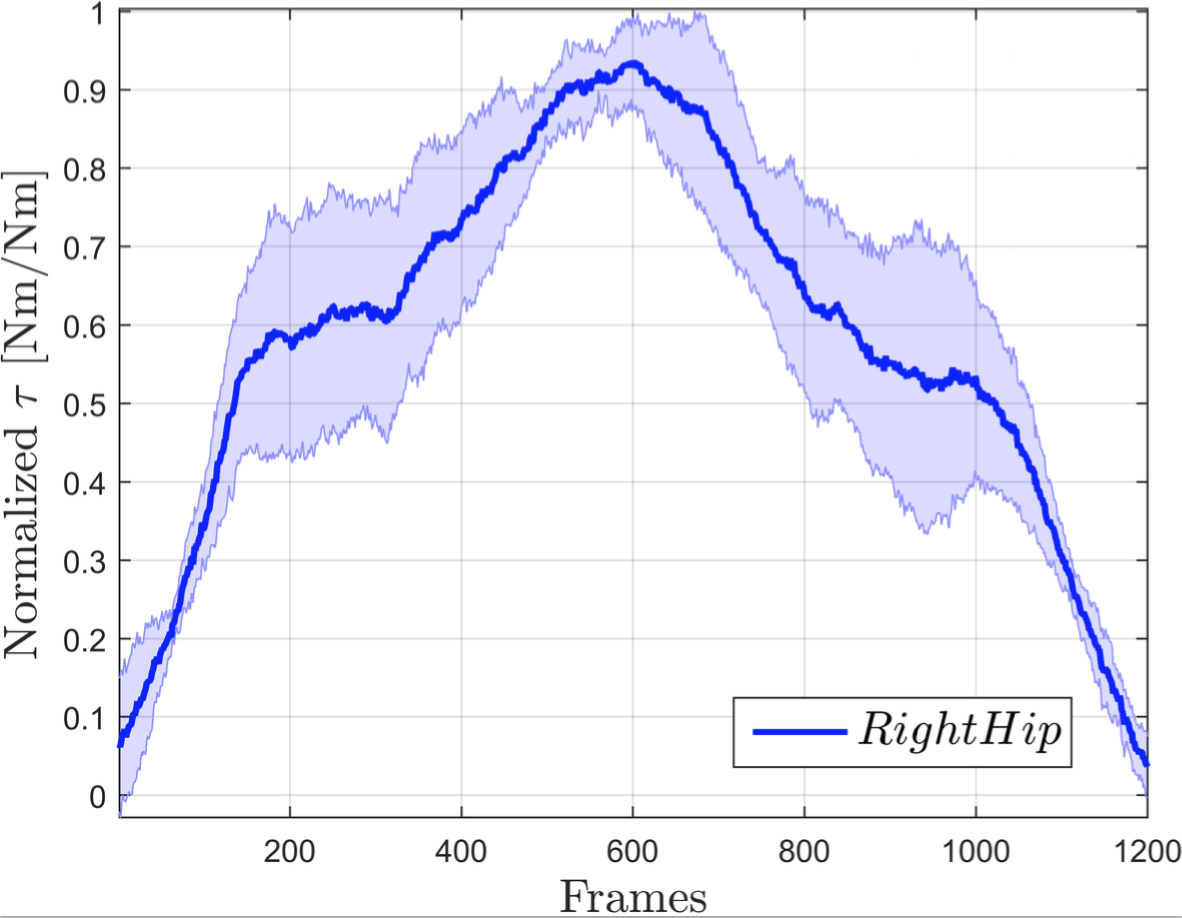
\includegraphics[width=0.48\textwidth]{figs/torqueRightHipBHR}
 %		\caption{}
 %		\label{fig:figs_torqueRightHipBRA}
 %	 \end{subfigure}
 %	\begin{subfigure}[b]{0.48\textwidth}                                                                 
   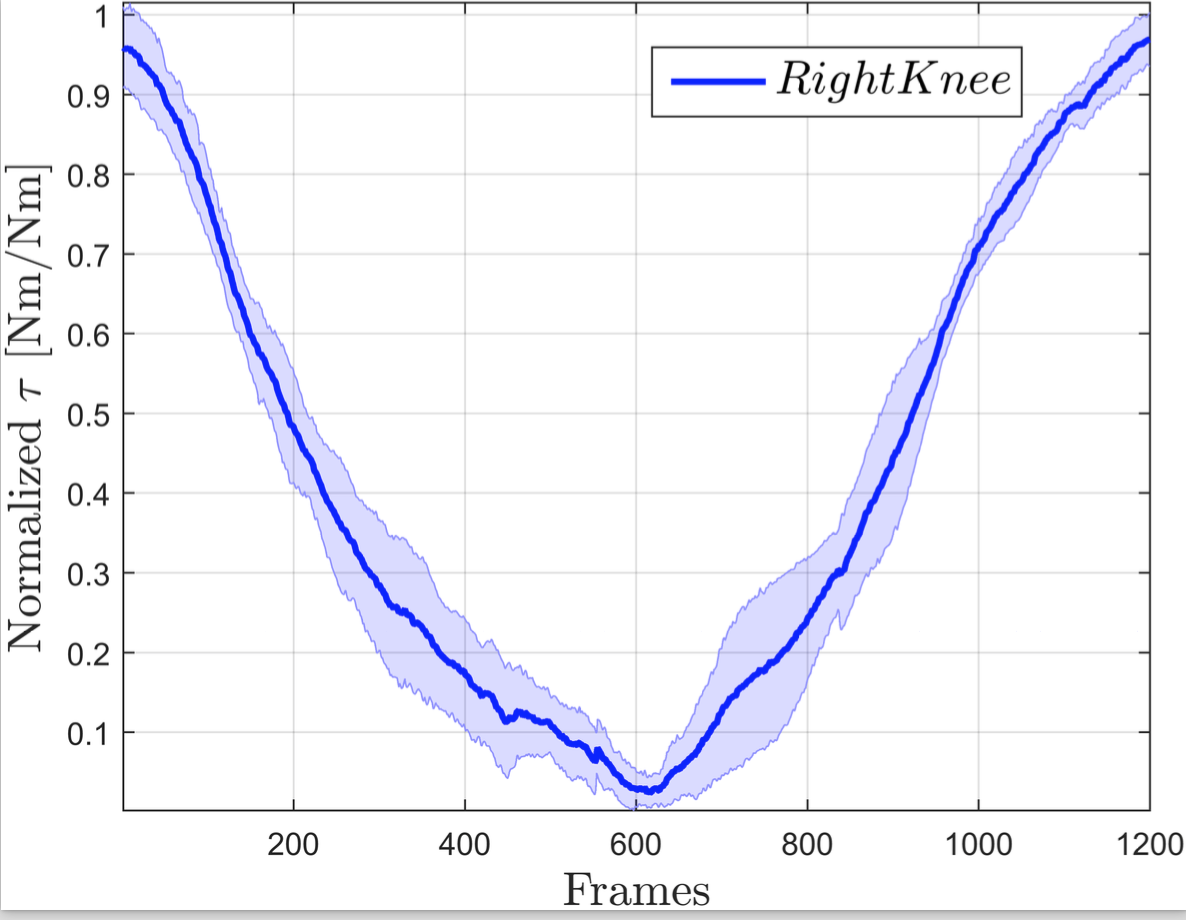
\includegraphics[width=0.48\textwidth]{figs/torqueRightKneeSH}
	%	 \caption{}
	%	\label{fig:figs_torqueRightKneeSH}
 %	 \end{subfigure}
 %	\begin{subfigure}[b]{0.48\textwidth}                                                         
 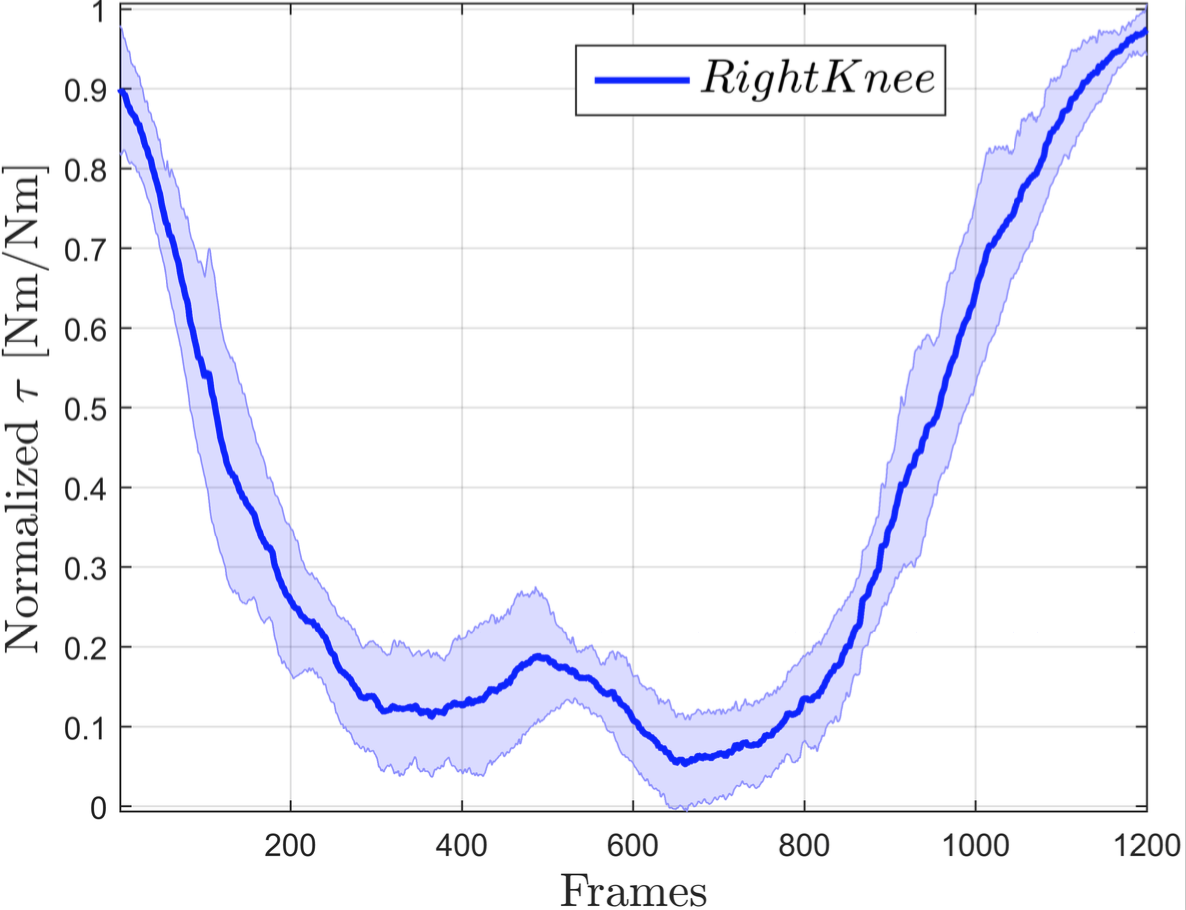
\includegraphics[width=0.48\textwidth]{figs/torqueRightKneeSHR}
 %		  	\caption{}
 	%	  	 \label{fig:figs_torqueRightKneeSR}
  %	 \end{subfigure}
      \caption{\emph{Inter-subjects analysis}: normalized torques of 10 subjects
		  (mean and standard deviation) for right hip in $BT$ without (a) and with (b) 
		  robot, for right knee in $ST$ without (c) and with (d) robot.}
 \end{figure*}
%
%%%%%%%%%%%%%%%%%%%%%%%%%%%%%%%%%%%%%%%%%%%%%%%%%%%%%%%%%%%%%%%%%%%%%%%%%%%%%%%%%%%%%%%%%%%%%%%%
\subsection{Robustness test}
To test the robustness of the method with respect to modeling errors we asked one subject to
perform the $BT$ with the robot in two different configurations, i.e. \emph{with} and
 \emph{without} an additional mass ($W$) of \unit{6}{\kilo}{\gram} roughly positioned in
  correspondence of the torso center of mass. The MAP computation was performed by
   considering as algorithm inputs the following cases (see Table \ref{table:robustness}):
	\begin{itemize}
		\item \emph{case A}: model of the subject without $W$ and measurements acquired 
		while performing the $BT$ with $W$;
		\item \emph{case B}: model of the subject without $W$ and measurements acquired 
		while performing the $BT$ without $W$.
		\end{itemize} 
Since in both the cases the analysis is performed with the model  of the subject without $W$, in
order to highlight a lower reliability for the model used in 
\emph{case A} computation, it is assigned a value to the model variance
\footnote{We refer here to the model covariance associated to the model as a diagonal matrix 
where each element of the diagonal is the variance value.}
 equal to $10^{-1}$ 
(different from the value of variance equal to $10^{-4}$ assigned for the \emph{case B}).
%
\begin{table}[H]
\caption{Cases for the MAP evaluation.}
\label{table:robustness}
\centering
\footnotesize
   \begin{tabular}{ l|| l | l | l | l | l | l | l | l  } 
    \multicolumn{1}{c||}{} &
    \multicolumn{3}{c|}{\emph{\textbf{case A}}} &
      \multicolumn{3}{c|}{\emph{\textbf{case B}}}\\
    \hline
	\hline
        \multicolumn{1}{|c||}{\emph{\textbf{model}}} &
    \multicolumn{3}{c|}{without W} &
      \multicolumn{3}{c|}{without W} \\
    \hline
    \multicolumn{1}{|c||}{\emph{\textbf{measurements}}} &
    \multicolumn{3}{c|}{with W} &
      \multicolumn{3}{c|}{without W}\\
	\hline
      \multicolumn{1}{|c||}{$\Sigma$ \emph{\textbf{model}}} &
      \multicolumn{3}{c|}{$10^{-1}$} &
        \multicolumn{3}{c|}{$10^{-4}$}\\
     \hline   
     % \hline
     \multicolumn{1}{|c||}{\emph{\textbf{MAP torque estimation}}} &
     \multicolumn{3}{c|}{$\bm \tau_{(model + \unit{6}{\kilo}{\gram})}$} &
       \multicolumn{3}{c|}{$\bm \tau_{model}$}\\
      \hline
    \end{tabular}
\end{table}
%
By exploiting the linearity property of the system we started by considering the 
following expression for the torques
\begin{eqnarray} \label{tauEq}
	\bm \tau_{(model + \unit{6}{\kilo}{\gram})} - \bm \tau_{model} = 
	\bm \tau_{\unit{6}{\kilo}{\gram}}
\end{eqnarray} 
where $\bm \tau_{\unit{6}{\kilo}{\gram}}$ is the theoretical torque due to the additional $W$
positioned on the torso\footnote{We consider a simple 2-DoF system (see \cite{LatellaSensors2016}) in which the position of $W$ and the hip joint angle are known.}.  Given \eqref{tauEq}, 
 it is possible to retrieve the error $\bm{\varepsilon}_{\bm{\tau}}$ on the $\bm \tau$ 
  estimation for the subject with $W$, due to \emph{case A}:
  %
\begin{eqnarray} \label{TorquesError}
	\bm{\varepsilon}_{\bm{\tau}} = |\bm \tau_{(model + \unit{6}{\kilo}{\gram})} -
	 \bm \tau_{model}| - \bm \tau_{\unit{6}{\kilo}{\gram}}
\end{eqnarray}
%
We computed \eqref{TorquesError} by using the OpenSim ID (Inverse Dynamics) toolbox 
as well, in order to evaluate its effectiveness with respect to the modeling errors.
Figures \ref{fig:MAPtau_cmp}-\ref{fig:OPENSIMtau_cmp} provide the mean and the standard deviation of the torque estimation by means of the MAP algorithm and the OpenSim software, respectively.  Figure \ref{fig:BOXPLOT} shows the comparison between the computation of the error in \eqref{TorquesError} for both the above methods: the error is higher in OpenSim computation than in MAP since OpenSim does not offer the possibility of setting the model reliability in the computation.
%
% \begin{figure}[h!]
%   \centering
%    \begin{subfigure}[b]{1\columnwidth}
%       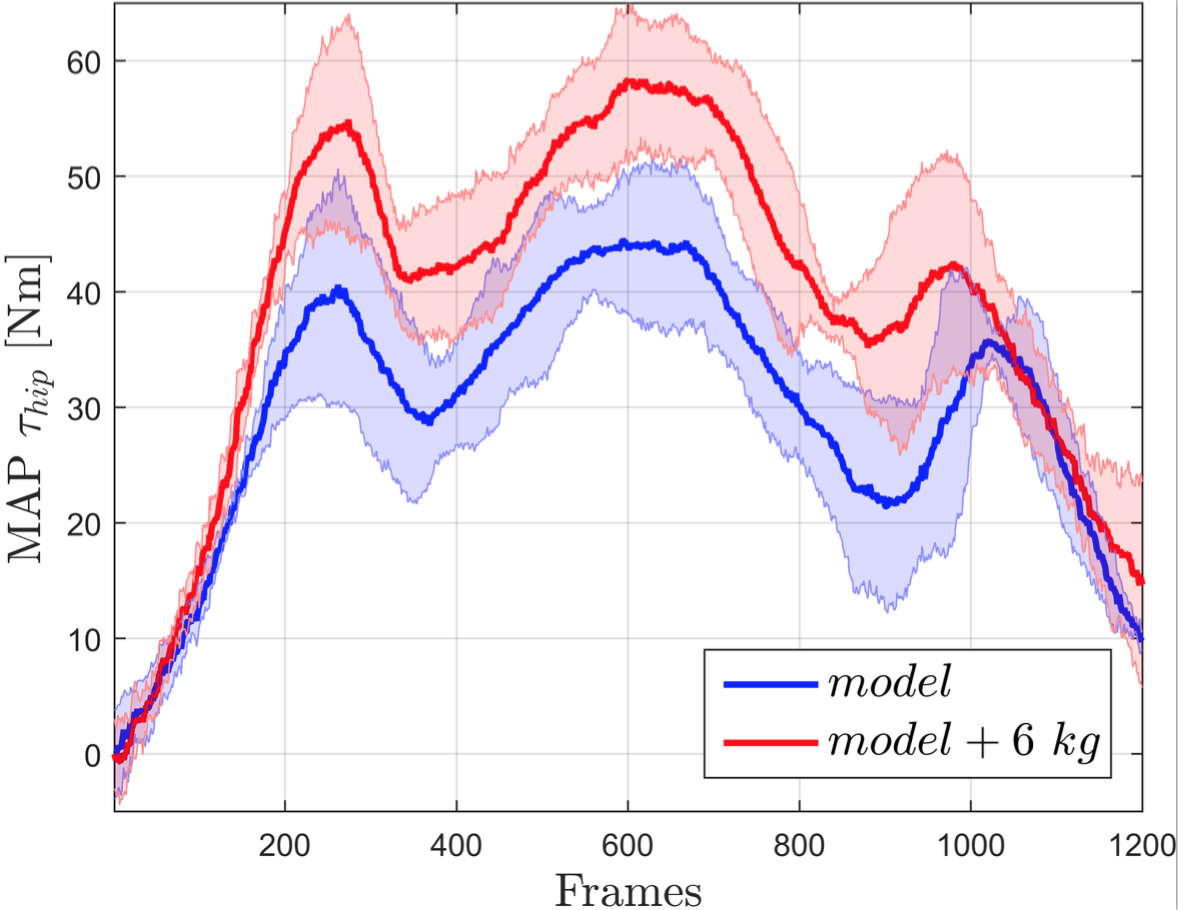
\includegraphics[width=\textwidth]{figs/TorqueComparison.pdf}
%           \caption{}
%           \label{fig:figs_torqueRightHipBH}
%   \end{subfigure}
%    \begin{subfigure}[b]{1\columnwidth}
%     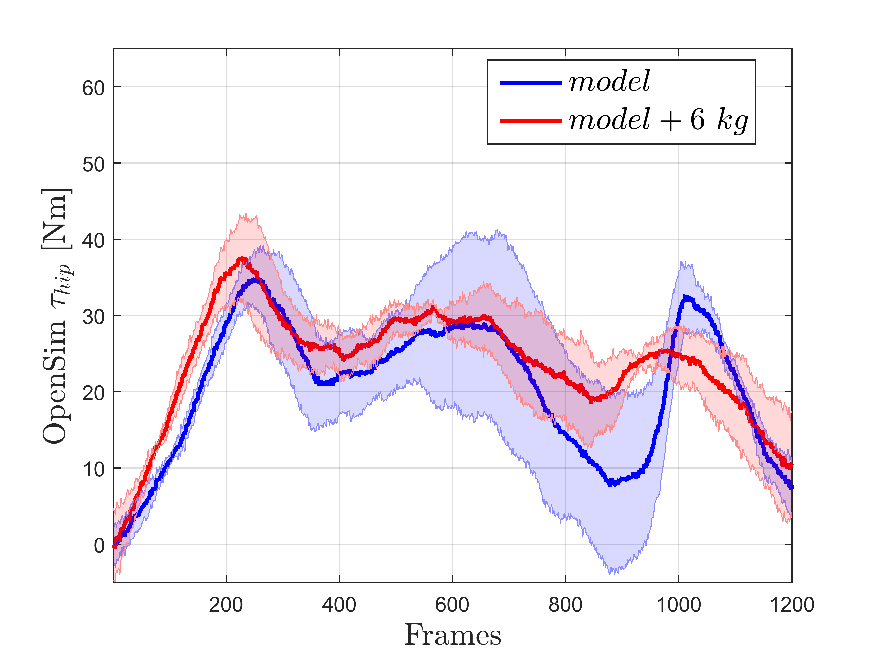
\includegraphics[width=\textwidth]{figs/TorqueComparisonOPENSIM.pdf}
% 	\caption{}
%         \label{fig:figs_torqueRightKneeSR}
%    \end{subfigure}
%           \caption{\emph{Intra-subjects analysis}: }
% \end{figure}
%
 \begin{figure*}[!ht]
	 \centering
%	\begin{subfigure}[b]{0.33\textwidth}
		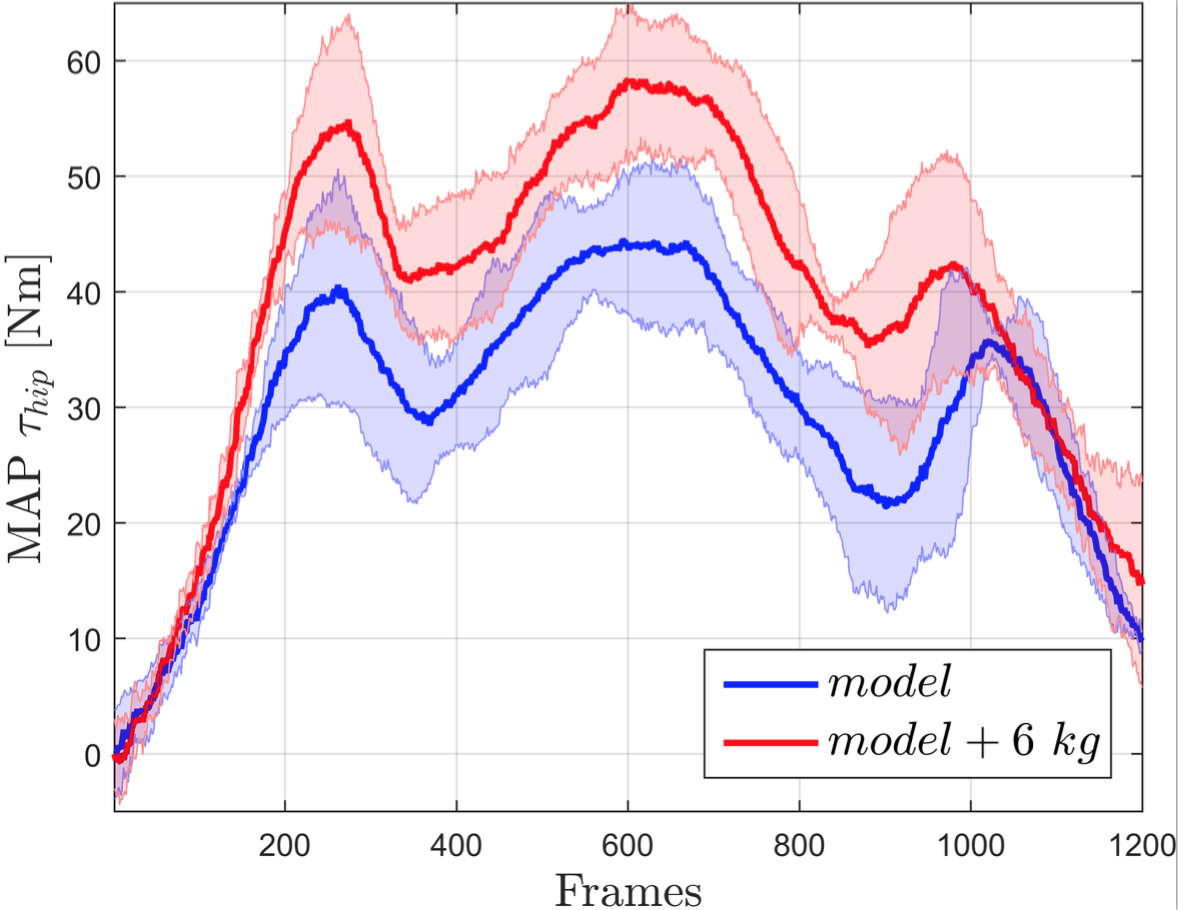
\includegraphics[width=0.3\textwidth]{figs/TorqueComparison}
%		\caption{}
%		\label{fig:MAPtau_cmp}
%	 \end{subfigure}
% 	\begin{subfigure}[b]{0.33\textwidth}
 		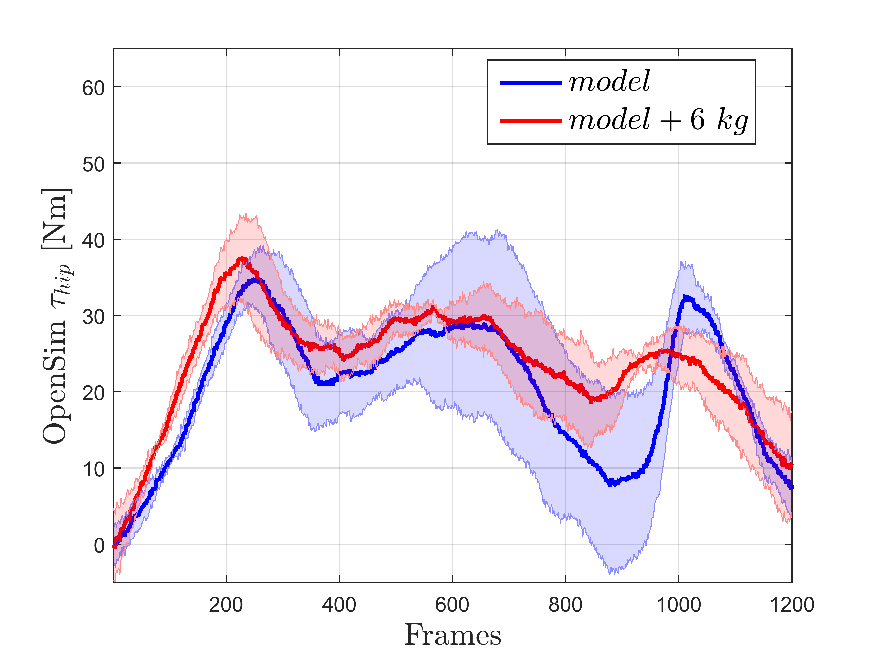
\includegraphics[width=0.3\textwidth]{figs/TorqueComparisonOPENSIM.pdf}
% 		\caption{}
%		\label{fig:OPENSIMtau_cmp}
% 	 \end{subfigure}
%  	\begin{subfigure}[b]{}
  		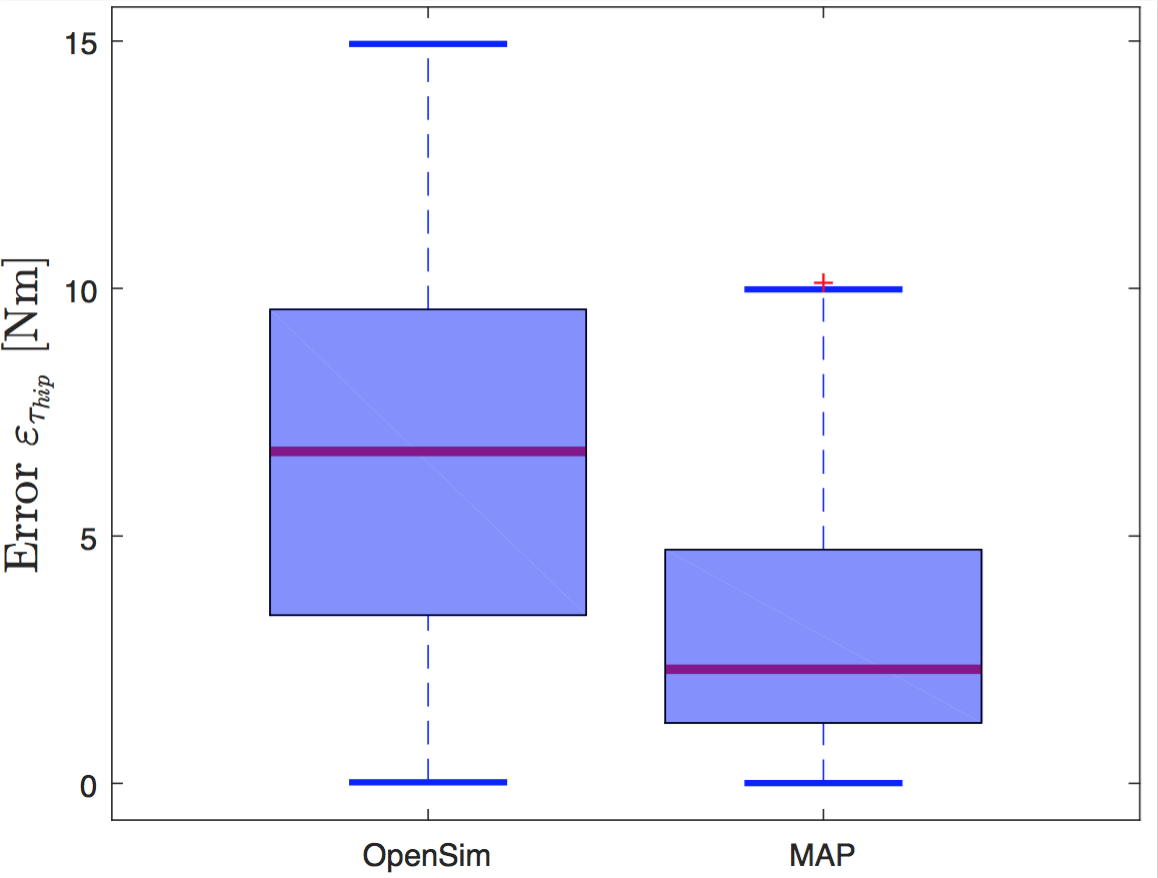
\includegraphics[width=0.3\textwidth]{figs/OPENSIMvsMAP}
%  		\caption{}
%		\label{fig:BOXPLOT}
%  	 \end{subfigure}
     \caption{\emph{Intra-subjects analysis}: mean and standard deviation of $\bm \tau$
	  (i.e., the sum of the $\bm \tau$ estimated at the hips)
	 among five repetitions of the $BT$ performed by a subject computed for \emph{case A} 
	 (red) and \emph{case B} (blue) by means of (a) MAP algorithm  and (b) by using the 
	 OpenSim ID (Inverse Dynamics) toolbox. (c) Box plots of the torque estimation error
	 $\bm{\varepsilon}_{\bm{\tau}}$ computed in \eqref{TorquesError} with MAP (on the right)
	 and with OpenSim (on the left). It shows that MAP is a method more robust to the
	 modelling errors since it gaves the possibility of weighting the reliability of the model
	  by properly setting the related covariance matrix. }
 \end{figure*}

%%%%%%%%%%%%%%%%%%%%%%%%%%%%%%%%%%%%%%%%%%%%%%%%%%%%%%%%%%%%%%%%%%%%%%%%%%%%%%%%%%%%%%%%%%%%%%%%
\subsection{Incremental sensor fusion analysis}
Since a distinctive feature of our framework consists in the possibility of building
 \eqref{eq:measRNEA} for different sources of measurement, we here investigate the advantage in
  using this algorithm for the dynamics estimation. We consider three sets of $\bm y$ 
  equations for: 
\begin{enumerate}
	\item  the two force plates: 
	\begin{eqnarray}
		\bm{y}_{\mbox{\scriptsize{\emph{FP}}}} & = & {}^{{\mbox{\scriptsize{\emph{FP}}}}}
		\bm{X}_{\mbox{\scriptsize{\emph{hFOOT}}}}~\bm{f}_{\mbox{\scriptsize{\emph{hFOOT}}}}
	\end{eqnarray}
	where it is used the trasformation matrix\footnote{See \cite{Featherstone2008}
	 for the definition of the trasformation
	 matrix between two reference frames.} $\bm X$  between the human foot reference frame 
	(${\mbox{\footnotesize{\emph{hFOOT}}}}$) and each force plate frame
	 (${\mbox{\footnotesize{\emph{FP}}}}$);
	\item  the IMUs embedded in the suit:
	\begin{eqnarray}
		\bm{y}_{\mbox{\scriptsize{\emph{IMU}}}} & = &
		 {}^{\mbox{\scriptsize{\emph{IMU}}}}\bm{X}_{\mbox{\scriptsize{\emph{L}}}}~
		 \bm{a}_{\mbox{\scriptsize{\emph{L}}}}
	\end{eqnarray}
	by exploiting the trasformation between each human link frame
	 ${\mbox{\footnotesize{\emph{L}}}}$ 
	on which the IMU is attached and
	that particular IMU reference frame (Fig. \ref{fig:figs_human_JointLink}a);  
	\item  the force/torque sensors of the two arms of the robot:
	\begin{eqnarray}
		\bm{y}_{\mbox{\scriptsize{\emph{iCubFT}}}} & = &
		 {}^{\mbox{\scriptsize{\emph{iCubFT}}}}\bm{X}_{\mbox{\scriptsize{\emph{hHAND}}}}~
		 \bm{f}_{\mbox{\scriptsize{\emph{hHAND}}}}
	\end{eqnarray}
	for which it is necessary knowing the transformation between each human hand frame
	(${\mbox{\footnotesize{\emph{hHAND}}}}$)
	to the robot sensor frame (${\mbox{\footnotesize{\emph{iCubFT}}}}$).
\end{enumerate}

\indent
A general overview of the above-mentioned frames is shown in Fig.
 \ref{fig:interaction_lateral&top}a. We want to prove that, by adding progressively 
 the different sensors data at each MAP computation, the variance associated to 
 the estimated dynamic variables consequently decreases, making the estimation more reliable.
%
In particular, we build \eqref{eq:measRNEA} for three different cases (Fig.
 \ref{fig:sensAddition&barAnalysis}a) :
\begin{itemize}
\item[\textit{case 1)}]  $\bm{y} = [\bm{\ddot{q}},~\bm{y}_{\mbox{\scriptsize{\emph{FP}}}}]$
\item[\textit{case 2)}] $\bm{y} = [\bm{\ddot{q}},~\bm{y}_{\mbox{\scriptsize{\emph{FP}}}},~ \bm{y}_{\mbox{\scriptsize{\emph{IMUs}}}}]$ 
\item[\textit{case 3)}] $\bm{y} = [\bm{\ddot{q}},~\bm{y}_{\mbox{\scriptsize{\emph{FP}}}},~ \bm{y}_{\mbox{\scriptsize{\emph{IMUs}}}},~\bm{y}_{\mbox{\scriptsize{\emph{iCubFT}}}}]$.
\end{itemize}
%
The MAP computation is performed for each case since the incremental addition of a sensor 
includes each time a new information on the analysis.  
For this analysis we take into account a task involving the robot ($BT$) in order to 
include the robot sensor measurements in the computation.  Among the variables in $\bm d$ we consider again the torque $\bm \tau$ (i.e., right and left ankle and hip) and the variance along the axis of major relevance $y$.

 \begin{figure*}[!ht]
	 \centering
		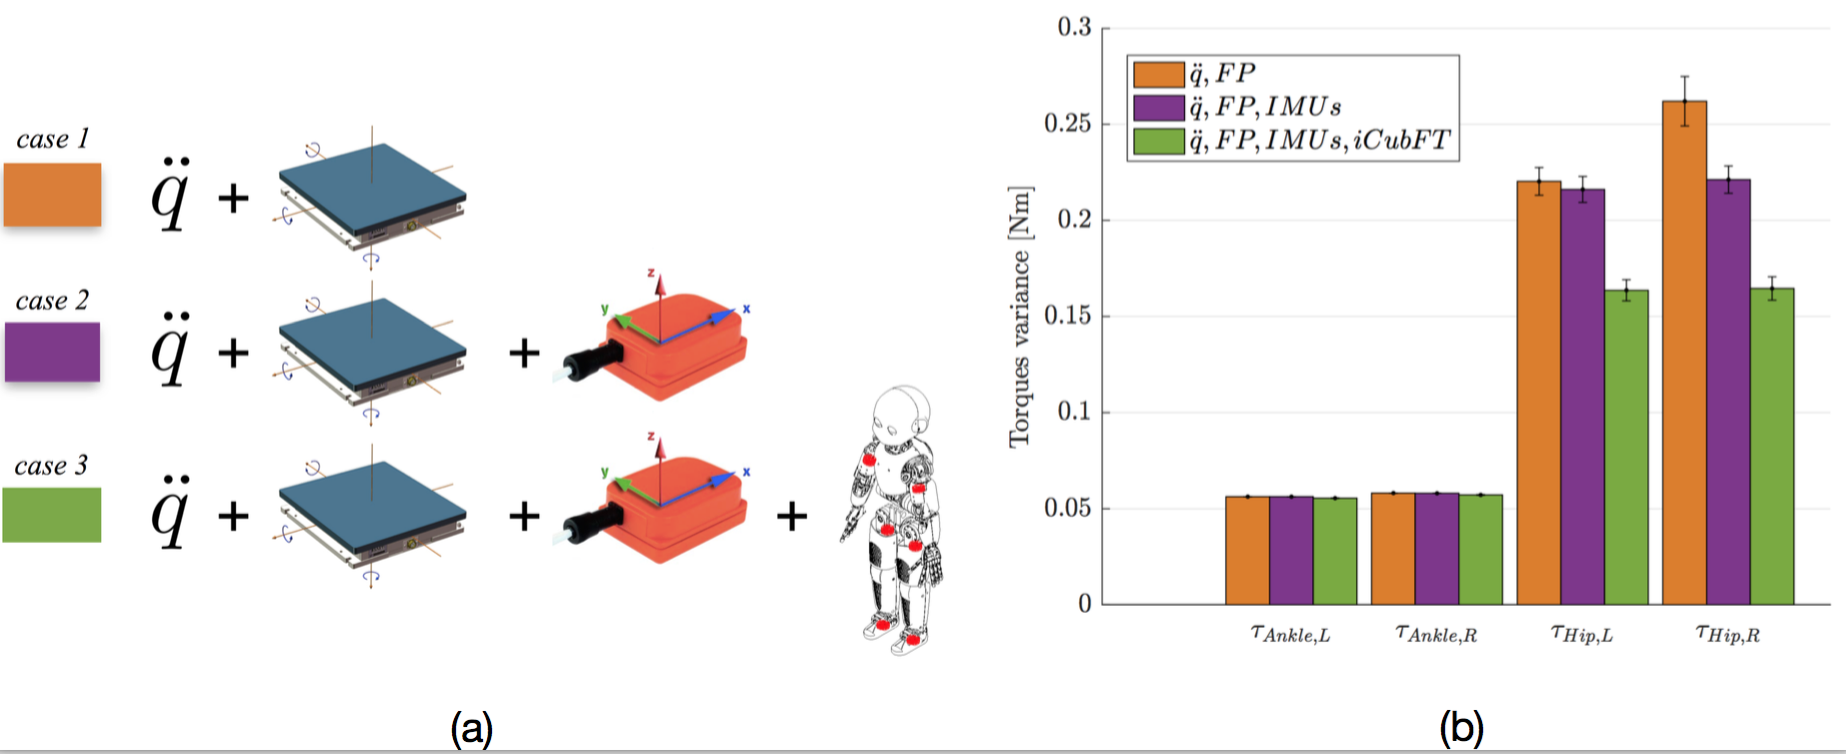
\includegraphics[width=0.9\textwidth]{figs/sensAdditionAndBarAnalysis}
      \caption{(a) Description of three cases for progressive addition of sensors.
	   (b) \emph{Inter-subjects analysis}: mean variance of $\bm \tau$ at the left and right
	    ankle and hip among five repetitions of the $BT$ performed by ten subjects computed 
		by MAP with the three different version of the measurements vector $\bm y$.}
		 		\label{fig:sensAddition&barAnalysis}
 \end{figure*}
% 
 % \begin{figure*}[h!]
 % 	 \centering
 % 	\begin{subfigure}[b]{0.48\textwidth}
 % 		\includegraphics[width=\textwidth]{figs/sensAddition.pdf}
 % 		\caption{}
 % 		\label{fig:figs_sensAdd}
 % 	 \end{subfigure}
 % 	\begin{subfigure}[b]{0.48\textwidth}
 % 		\includegraphics[width=\textwidth]{figs/SDall.pdf}
 % 		\caption{}
 % 		\label{fig:figs_SDall}
 % 	 \end{subfigure}
 %      \caption{(a) Description of three cases for progressive addition of sensors.
 % 	   (b) \emph{Inter-subjects analysis}: mean variance of $\bm \tau$ at the left and right
 % 	    ankle and hip among five repetitions of the $BT$ performed by ten subjects computed
 % 		by MAP with the three different version of the measurement vector $\bm y$.}
 % \end{figure*}
 %
Passing progressively from \textit{case 1} to \textit{case 3} (Fig. \ref{fig:sensAddition&barAnalysis}a)
the variance associated to the torques decreases\footnote{In order to assess 
the statistical significance of results, a paired-samples
 \emph{t-test} is performed firstly between \textit{case 1} and \textit{case 2} 
 ($2$ sensors vs $3$ sensors) and then between \textit{case 2} and \textit{case 3} 
 ($3$ sensors vs all sensors).  Torque variances statistically significant,  
  \emph{p-value} $<0.05$.}. In Fig. \ref{fig:sensAddition&barAnalysis}b we show 
the decreasing behaviour of the mean variance of the torque at the hips and at the ankles
 computed between ten subjects.
%
The variance values on the ankles do not change significantly among the three different
 configurations of sensors since the ankle torque estimation depends mostly on the 
 contribution of the force plates that are included in all the three 
 cases of the computation.  Conversely, a significant decreasing behaviour is present 
 in the values associated to the hips. In this case the contribution of the three sources 
 of sensors becomes important since the torque estimation at the hips are affected 
 by the all sensors.
 %!TEX root = ../template.tex

%%%%%%%%%%%%%%%%%%%%%%%%%%%%%%%%%%%%%%%%%%%%%%%%%%%%%%%%%%%%%%%%%%%%%%%%%%%%%%%%

\section{Physical human-robot interaction in Gazebo: lifting the iCub arm}

To test the control software for the robot lifting with the help of the human, we first realized a prototype application in Gazebo. In this application, the robot can lift from a chair autonomously or with the help of a human; to realize a physical interaction between the human (operator, in this case) and the robot simulated in Gazebo, we used the Geomagic touch, a haptic device.

The setup consists of:
\begin{itemize}
\item the iCub simulation in Gazebo, complete of the dynamics information provided by \textit{wholeBodyDynamicsTree} (\url{https://github.com/robotology/codyco-modules/tree/master/src/modules/wholeBodyDynamicsTree} developed by IIT in WP1) and the Cartesian information provided by \textit{iKinCartesianController};
\item the Geomagic Touch, installed following the instructions in \url{https://github.com/inria-larsen/icub-manual/wiki/Installation-with-the-Geomagic-Touch}, which not only install the SDK and drivers of the GeoMagic but also point to how to create the yarp drivers for the Geomagic;
\item a C++ module (\url{https://github.com/inria-larsen/icubLearningTrajectories}) that connects the output command from the Geomagic to the iCub in Gazebo, and eventually enables recording the trajectories on a file.
\end{itemize}

The interconnection among the different modules is sketched in Figure~\ref{fig:systemHaptic}.
The tip of the Geomagic is virtually attached to the end-effector of the robot:
$$ x_{geo} \rightarrow x_{icub\_hand} $$
When the operator moves the Geomagic in the space, the position of the Geomagic tip $x_{geo}$ is scaled (1:1 by default) in the iCub workspace as $x_{icub\_hand}$, and the Cartesian controller is used to move the iCub hand around a "home" position, or default starting position:
$$ x_{icub\_hand} = hapticDriverMapping(x_0 + x_{geo})$$
where the \textit{hapticDriverMapping} is the transformation applied by the haptic device driver, which basically maps the axis from the Geomagic reference frame to the iCub reference frame.
By default, no force feedback is sent back to the operator in this mode, as it emulates the zero-torque control pHRI where the robot is ideally transparent and not opposing any resistance to the human guidance. A default orientation of the hand ("katana" orientation) is set.

\begin{figure}[h]
\centering
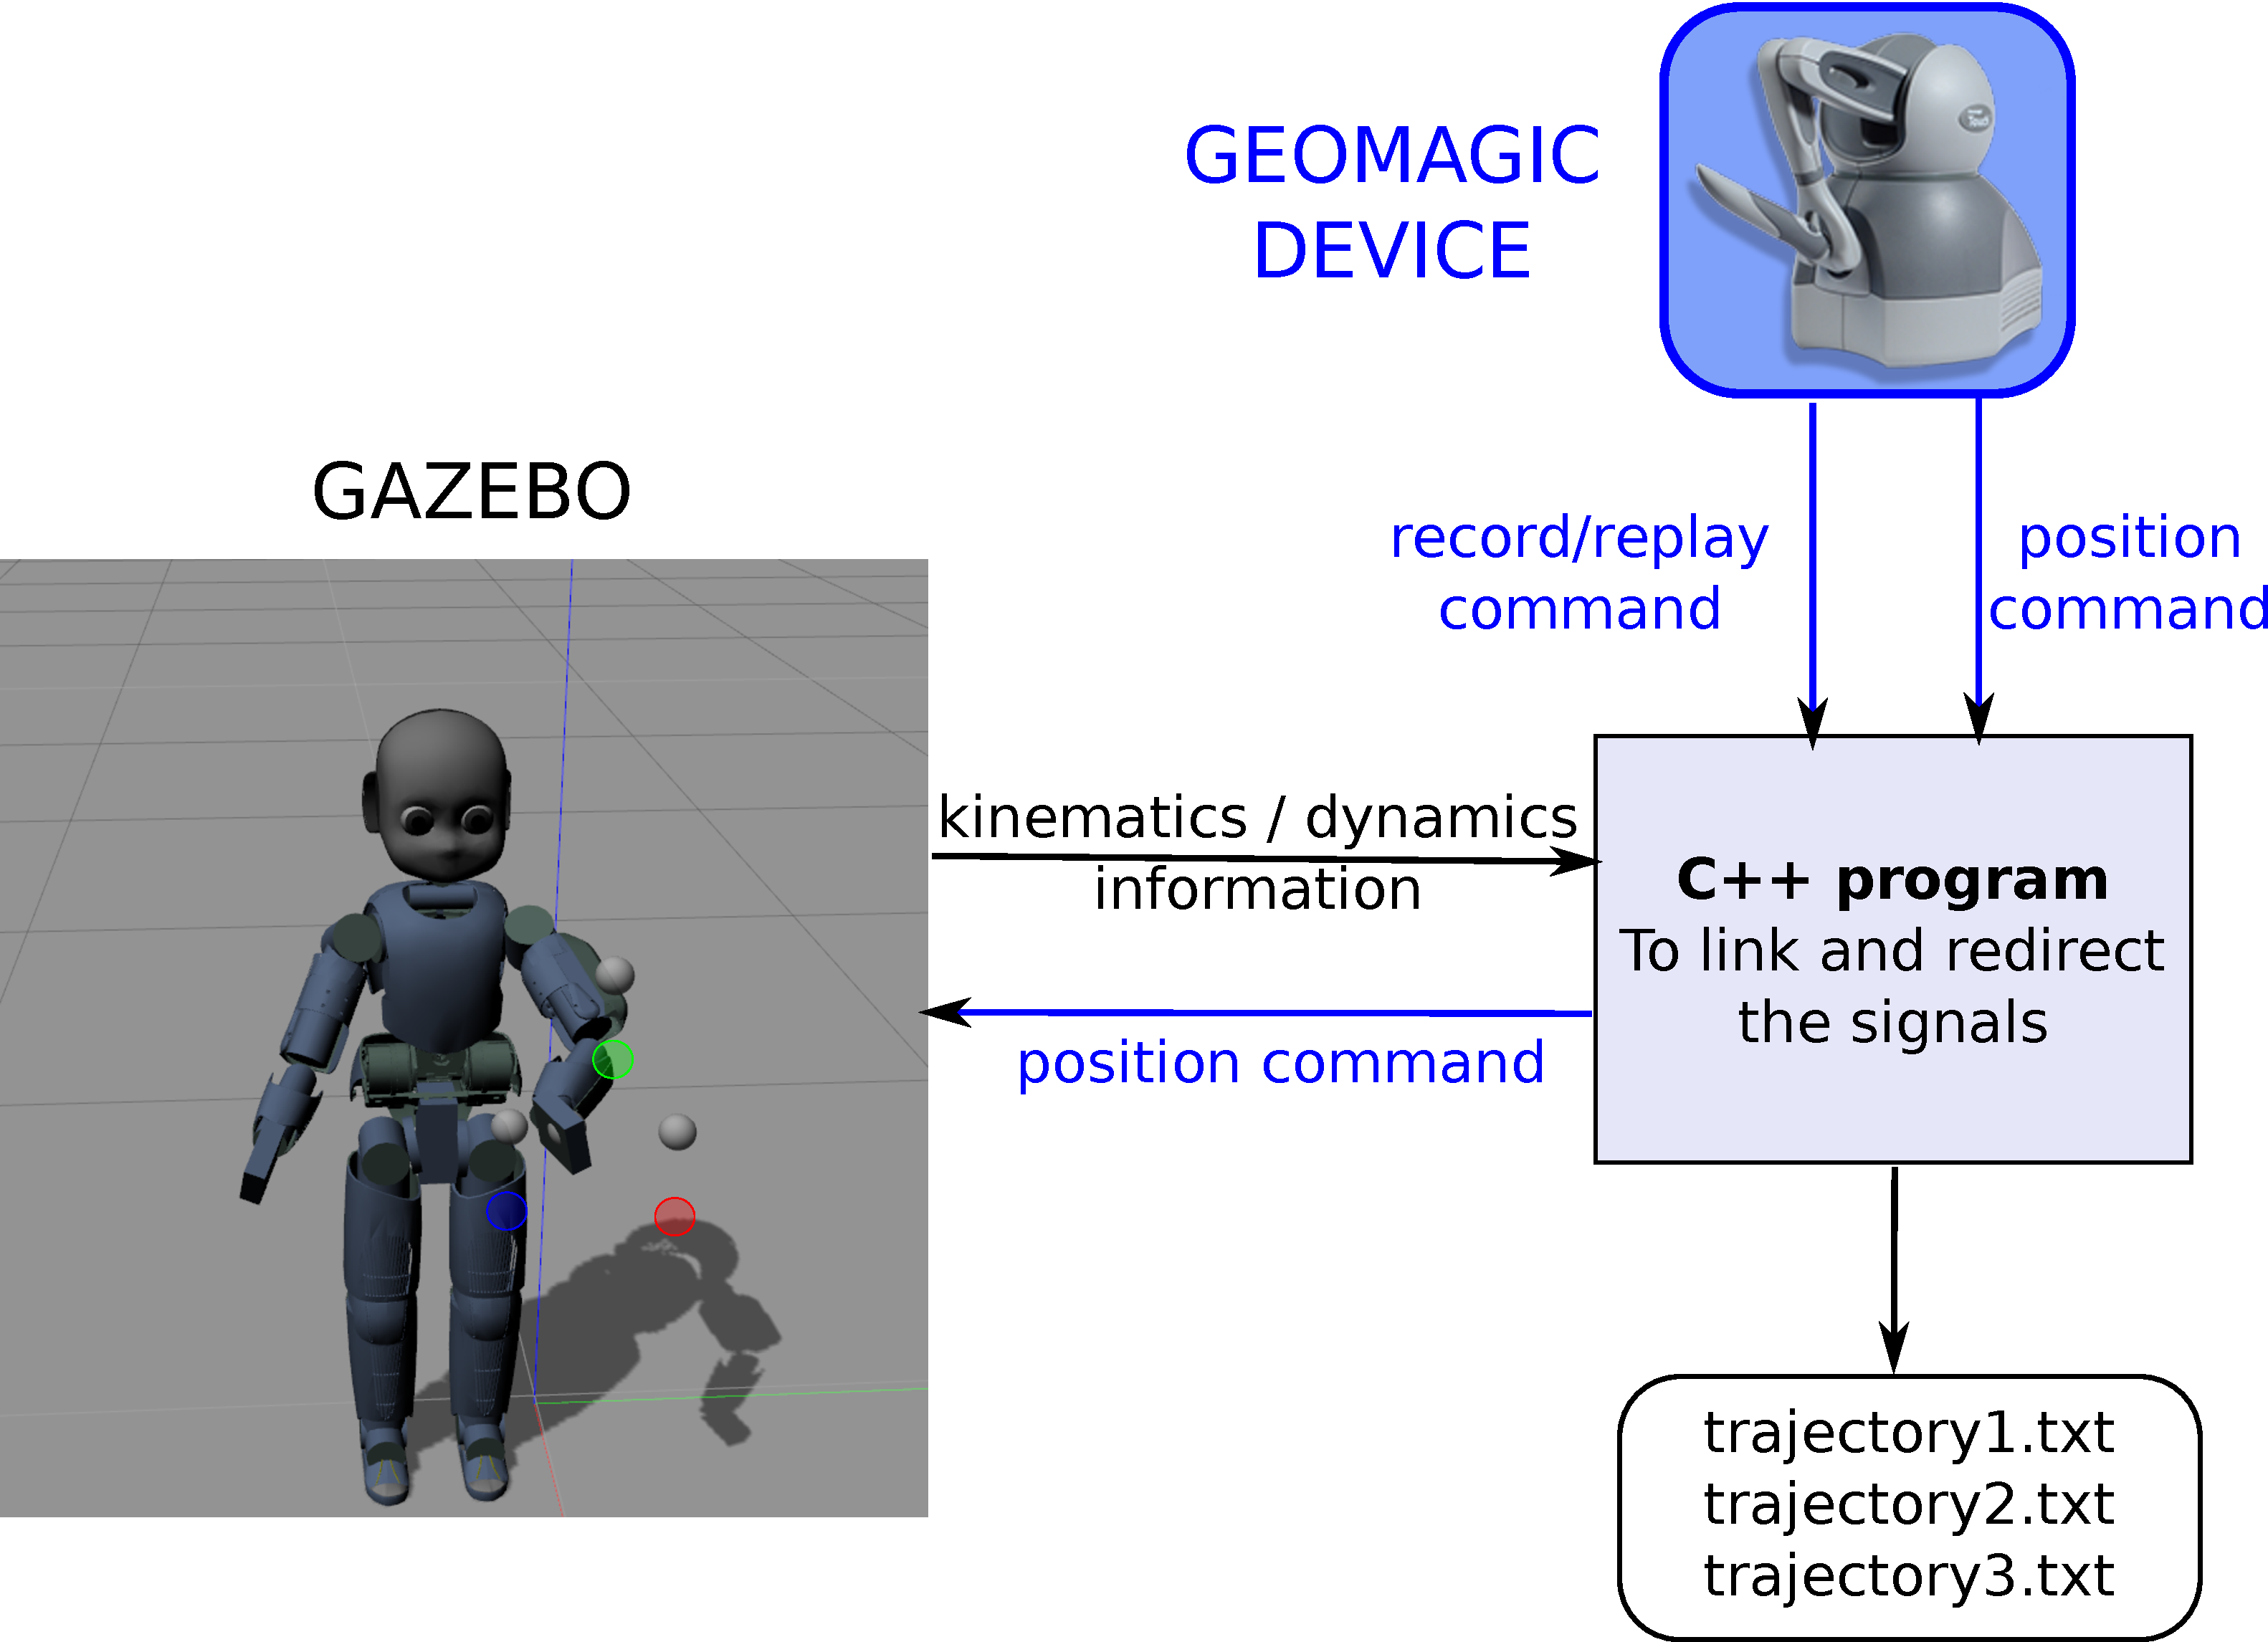
\includegraphics[height=7cm]{figs/geomagic_setup.pdf}
\caption{The interconnection between the Geomagic Touch and iCub in Gazebo.}
\label{fig:systemHaptic}
\end{figure}

The two buttons of the Geomagic are used to enable recording and replaying the trajectories (see Figure~\ref{fig:geobuttons}). To record a trajectory, the operator must click and hold the black button of the Geomagic; releasing the button stops recording the trajectory, and the trajectory is saved on a file (e.g., \textit{trajectory.txt}). To replay one of the trajectories from the $N$ previously recorded, the operator must click the light grey button of the Geomagic and then enter the number of the trajectory on the terminal.

\begin{figure}[h]
\centering
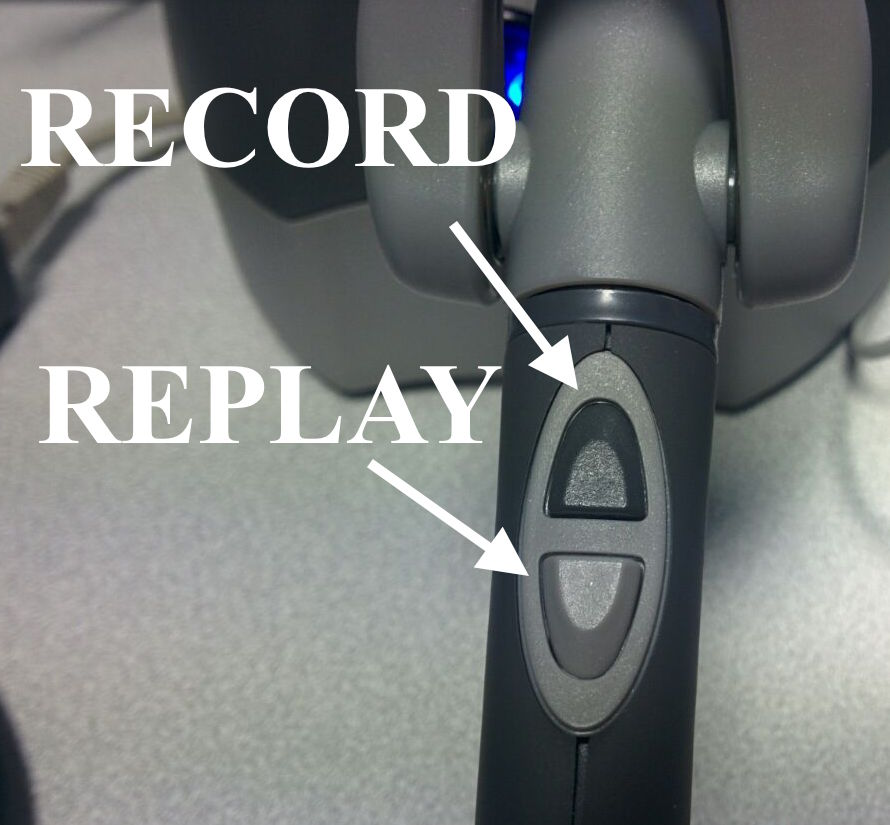
\includegraphics[height=5cm]{figs/geomagic_buttons.jpg}
\caption{The two buttons of the Geomagic.}
\label{fig:geobuttons}
\end{figure}

A video showing the iCub moved by the haptic device in Gazebo is available at this link: \url{https://www.youtube.com/watch?v=4ShyNtKojy0&feature=youtu.be}.
The graph in Figure~\ref{fig:trajectories} shows some trajectories recorded from the geomagic, corresponding to lifting the left arm of the iCub: the Cartesian position of the hand in the reference frame of iCub is shown.
\begin{figure}[h]
\centering
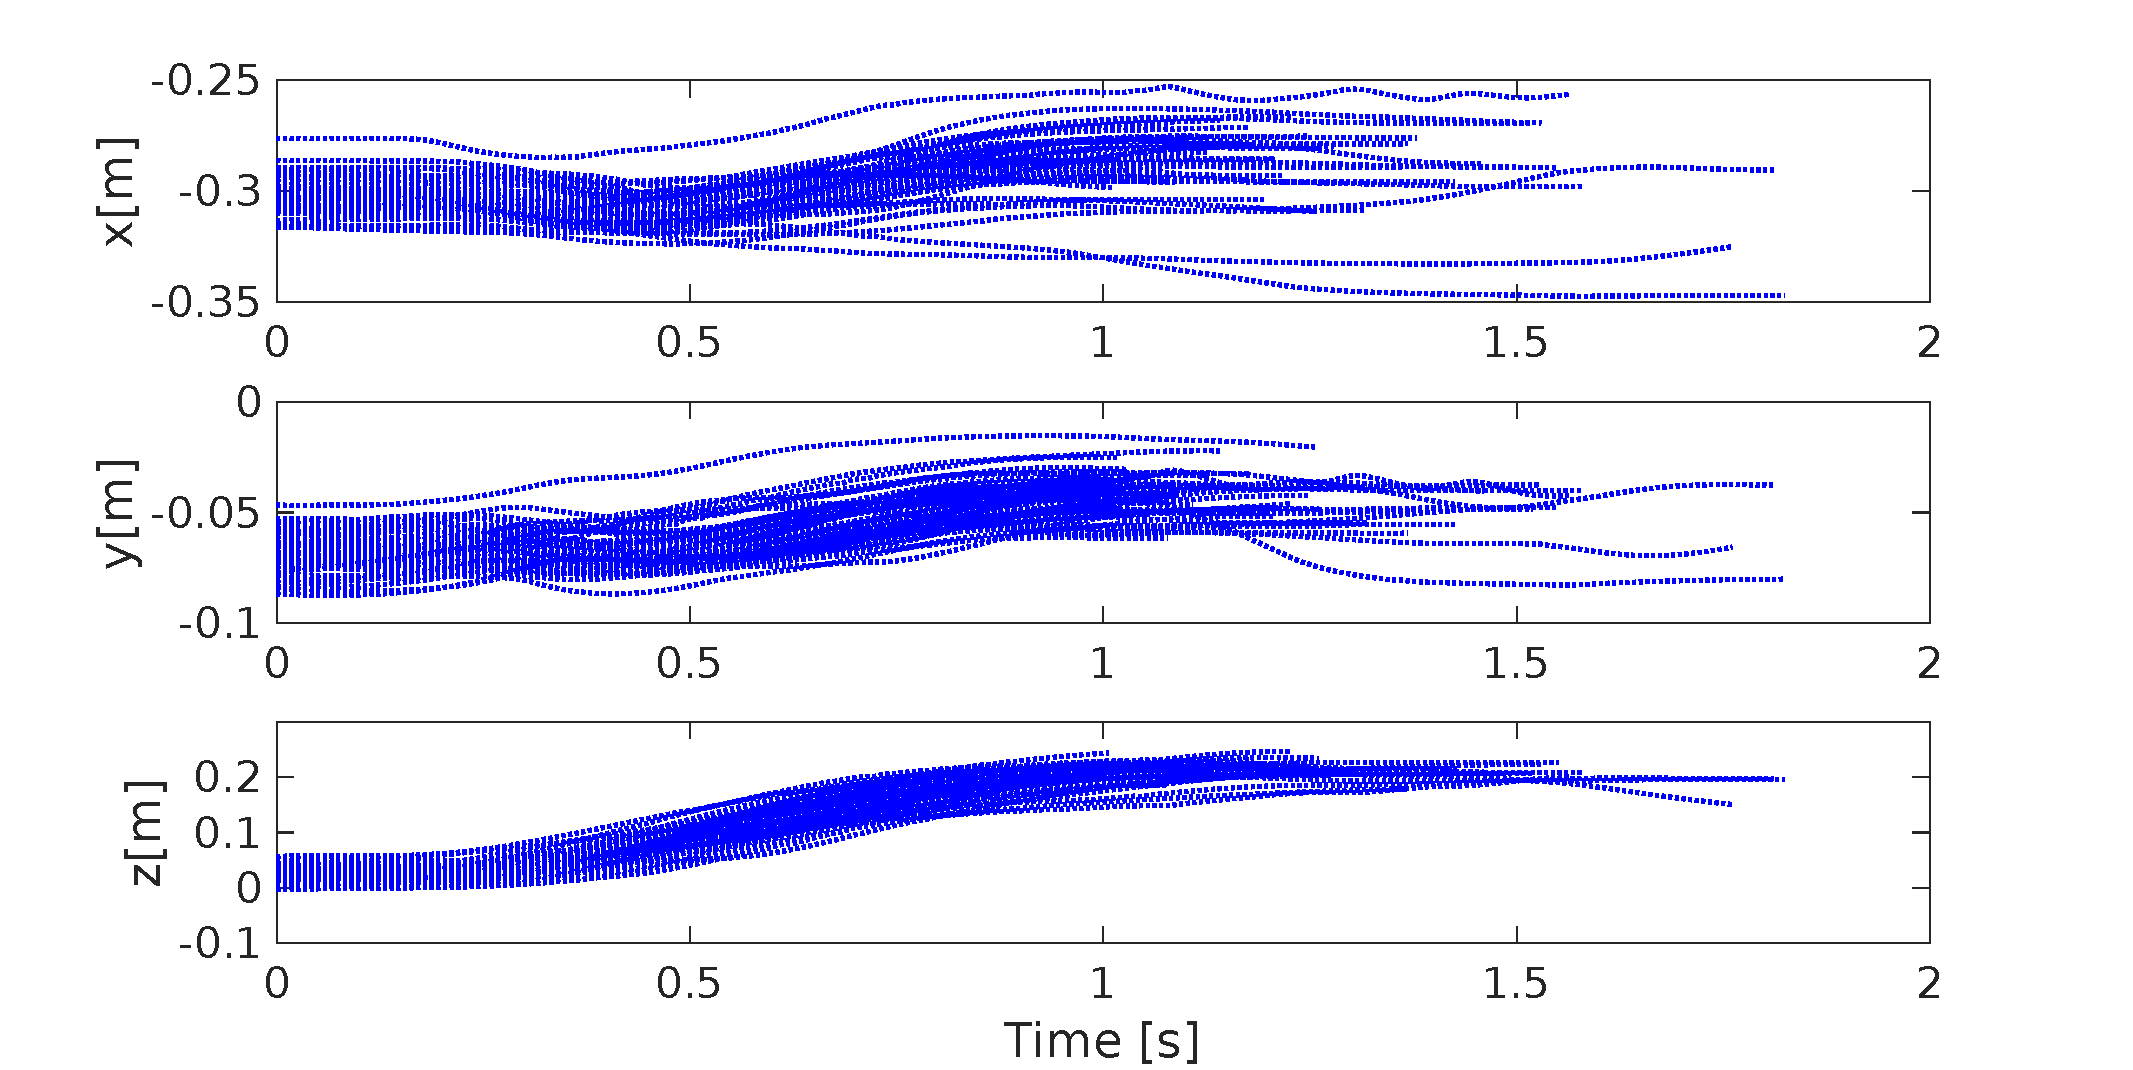
\includegraphics[height=7cm]{figs/geomagic_lifting_trajectories.pdf}
\caption{Some trajectories recorded when the geomagic is used to lift the left arm: Cartesian position of the end-effector.}
\label{fig:trajectories}
\end{figure}

Demonstrated trajectories and their corresponding forces can be recorded directly from the robot, by accessing the Cartesian interface and the Cartesian end-effector wrench computed by \textit{wholeBodyDynamicsTree}.

To enable a quicker visualization of the torques and forces in action on the robot during physical interaction (in both simulation and on the real robot) we developed some visualization GUI tools \url{https://github.com/inria-larsen/icub-wholebody-visualization}.
A major aim is to alert users, in real-time, when excessive torques are applied in one or more joints. This is especially needed when complex interactions take place between the robot, users and the environment, such as in the case of the robot being lifted from the chair.

 
%%%%%%%%%%%%%%%%%%%%%%%%%%%%%%%%%%%%%%%%%%%%%%%%%%%%%%%%%%%%%%%%%%%%%%%


\subsection{Learning a ProMP of the lifting movement}

Once we record a set of trajectories, we can learn the distribution of these demonstration in the form of a probabilistic movement primitive (ProMP) \cite{Paraschos_NIPS_2013a}.
Our toolbox for generating the proMP is currently written in Matlab, and available at \url{https://github.com/inria-larsen/icubLearningTrajectories}.

Let us consider the $n$ recorded trajectories \textcircled{$ \tau$} $= \{\tau_1,..., \tau_n \}$, where  the $i$-th trajectory is $\tau_i = \{y(t_1), ..., y(t_{f_i})\}$. 
$y(t)$ is the vector containing all the variables used to learn the ProMP, the simplest case being the mono-dimensional ProMP. If we want to learn the ProMP of the lifting motion (see Figure \ref{fig:trajectories}), the simplest case is $y(t) =\begin{bmatrix} z\end{bmatrix}^{\top}$, that is the $z$-axis Cartesian coordinate of the end-effector. You may notice that the duration of all the trajectories can be different, i.e.,  $t_{f_i}$ may be variable across demonstrations. 
To be able to find a common representation in term of primitive, a temporal modulation of the trajectories is applied, such that they all have the same number of samples $\bar{s}$. 

The ProMP is a Bayesian parametric model of the demonstrated trajectories in the form: 
$$y(t) = \Phi(t)^\top \omega + \epsilon_y$$ 
where $\Phi$ are $m$ radial basis functions scattered across time, scaled by the parameters vector $\omega \in R^m$. 
$\epsilon_y \sim \mathcal{N}(0, \beta) $ is the trajectory noise. 

For each $i$-th trajectory $\tau_i$, we compute the $\omega_i$ parameters vector:
$$y_i(t) = \Phi(t)^\top \omega_i + \epsilon_y$$ 
by minimizing the error between the observed trajectory $y_i(t)$ and its model $\Phi(t)^\top \omega_i + \epsilon_y$. This is done using the Least Mean Square algorithm, i.e.:
$$ \omega_i = (\Phi(t)^\top\Phi(t))^{-1}\Phi(t)^\top y_i(t).$$

Then, using the aggregated $[\omega_1,..., \omega_n]$ parameters, we can compute the distribution over these parameters $\omega \sim \mathcal{N}(\mu_\omega, \Sigma_w)$, and from this distribution, compute the distribution of the observed trajectories, which is the ProMP.

Figure \ref{fig:proMPlifting} shows the ProMP for the lifting motion, computed with the number of reference samples $\bar{s}=100$, number of basis functions $m=5$; the center of each RBF is equally distributed between 1 and $\bar{s}$.


\begin{figure}[h]
\centering
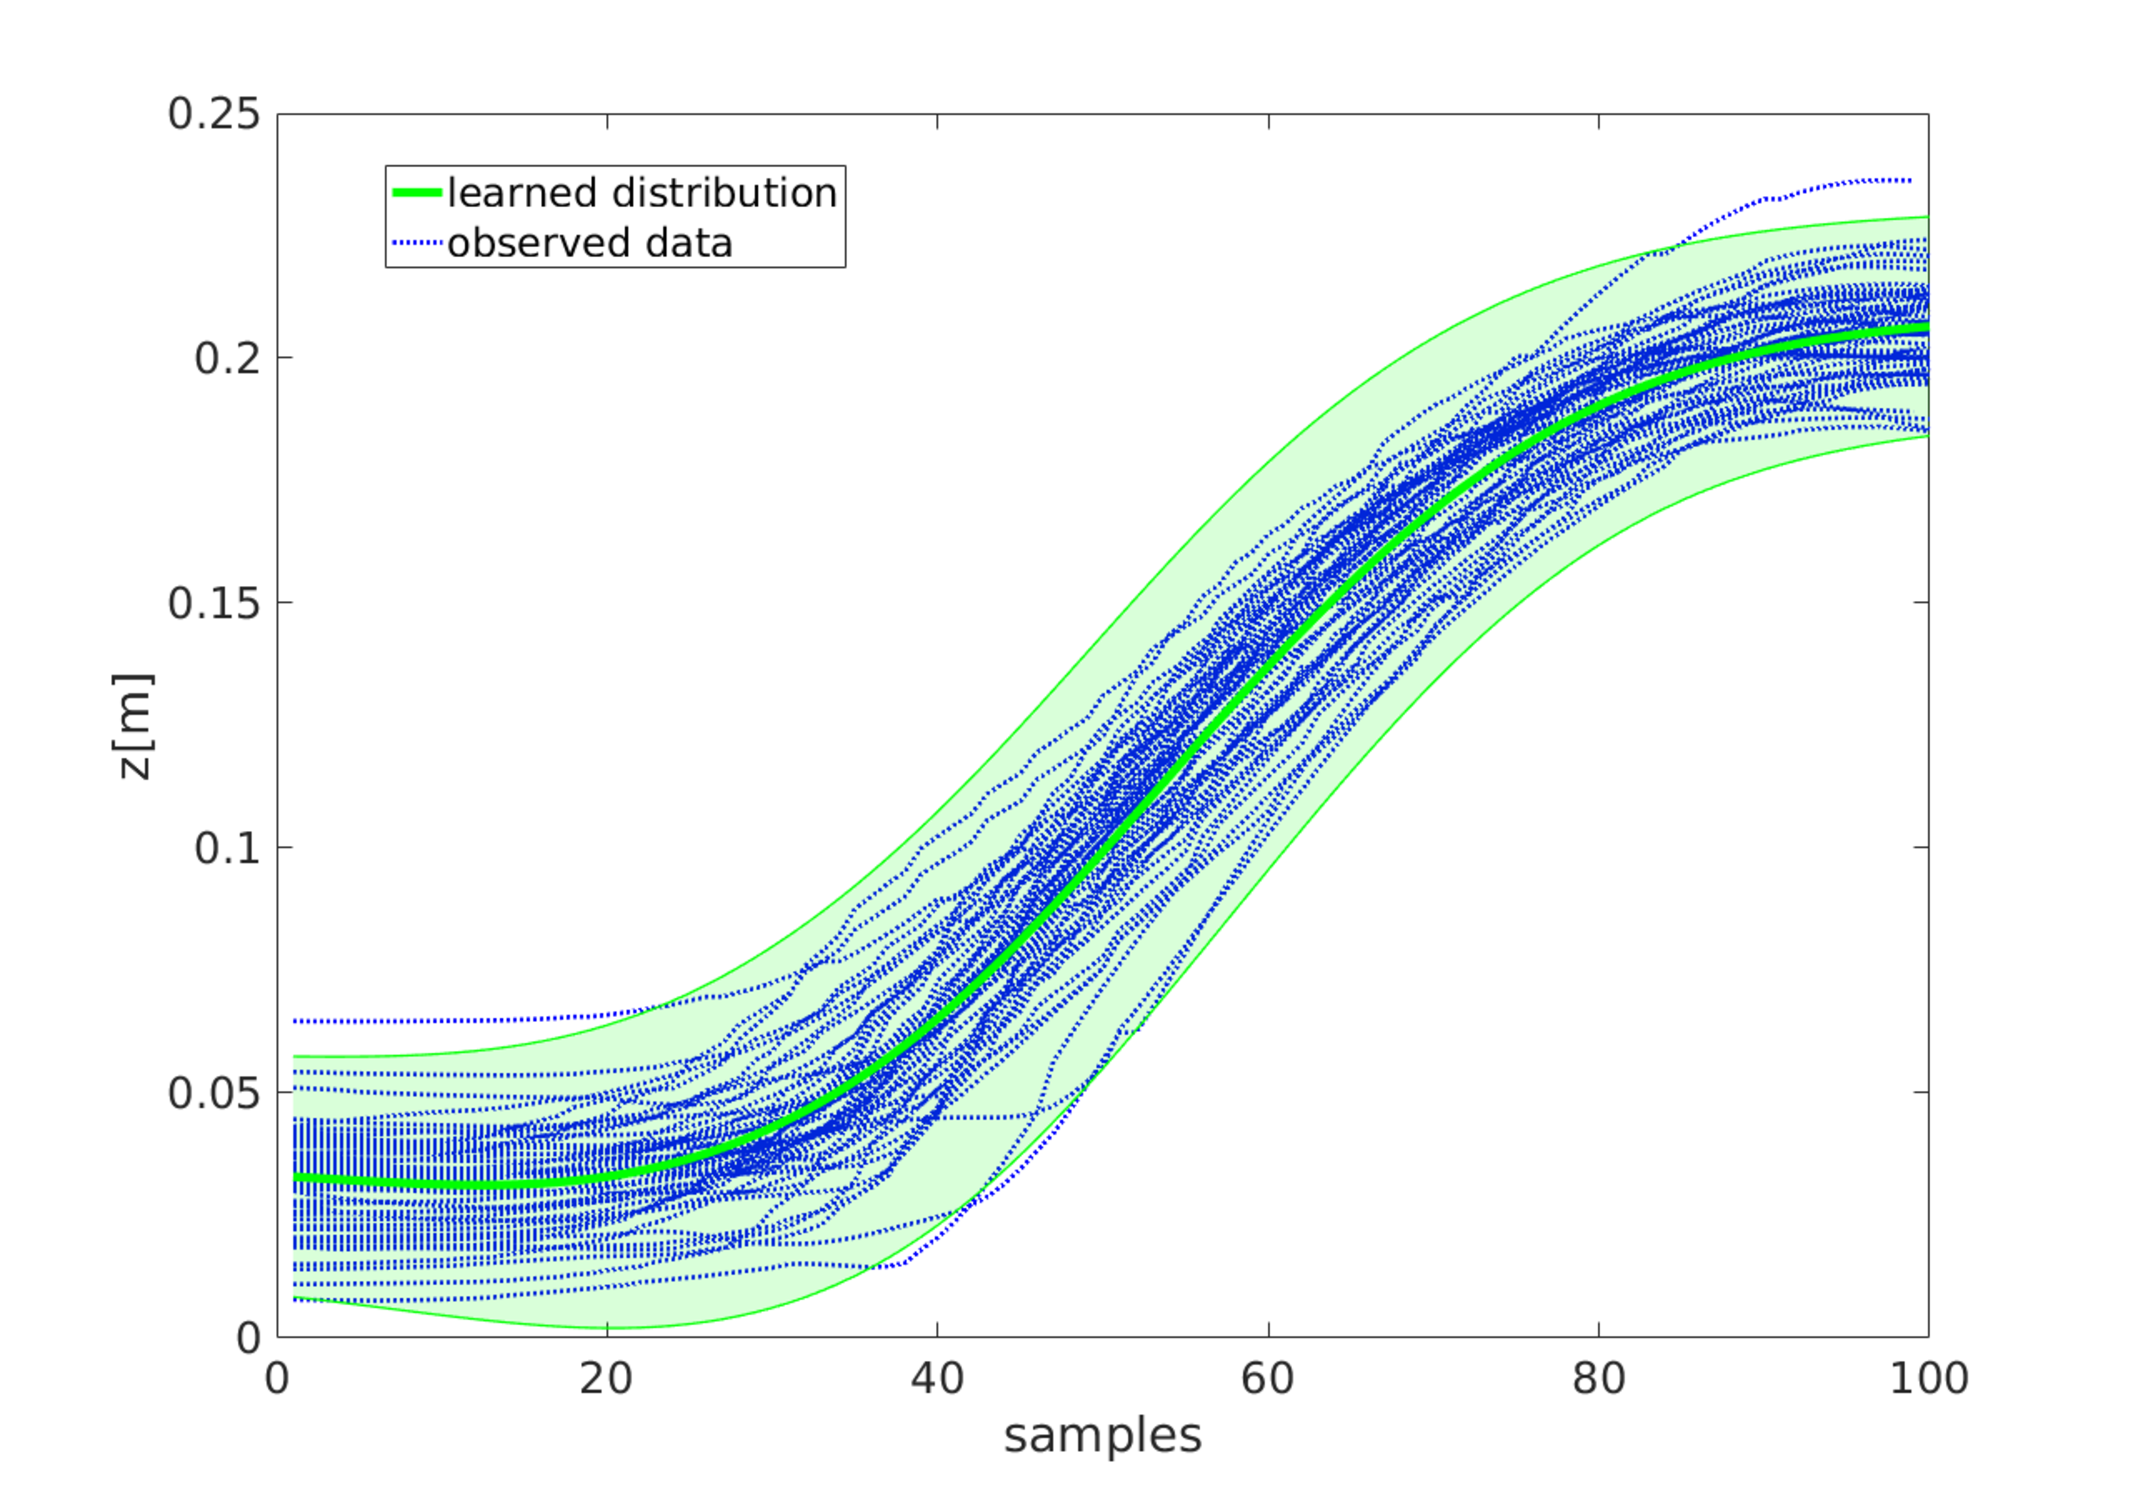
\includegraphics[height=9cm]{figs/proMPz.pdf}
\caption{proMP of the left end-effector $z$ coordinate when the arm is being lifted.}
\label{fig:proMPlifting}
\end{figure}





%%%%%%%%%%%%%%%%%%%%%%%%%%%%%%%%%%%%%%%%%%%%%%%%%%%%%%%%%%%%%%%%%%%%%%%
\subsection{Predicting the movement from initial observations}

Once the ProMP of a certain gesture has been learned (i.e., we have computed $\omega$ from $\omega_1, \ldots, \omega_n$), we can use it to predict the evolution of a movement just after few observations. Of course, the underlying hypothesis is that the movement that is observed ``belongs" to the distribution of demonstrated trajectories.

Let us consider the ProMP with the parameters distribution $\omega \sim \mathcal{N}(\mu_\omega, \Sigma_\omega)$.  

Suppose that we have $n_o$ observations of the trajectory to predict (e.g., lifting the arm), called 
$$D=[y^o(t_1),\ldots, y^o(t_{n_o})].$$

Our goal is to predict the evolution of the trajectory after $t_{n_o}$, i.e., find $\hat{y}(t_{n_o+1}),\ldots,\hat{y}(\hat{t}_f)$, where $\hat{t}_f$ is the estimate of the trajectory duration (by default the mean of all the $t_{f_1}, \ldots, t_{f_n}$). 
This is equivalent to predicting the entire trajectory $\hat{\tau}$ where the first $n_o$ samples are known and equal to the observations: $\hat{\tau} = \{y^o(t_{1}), ..., y^o(t_{n_o}), \hat{y}(t_{n_o+1}), ..., \hat{y}(t_{\hat{t}_f})\}$.
Therefore, our prediction problem consists in predicting $\hat{\tau}$ given the $D$ observations. Since $\hat{\tau}$ is computed by a ProMP, finding $\hat{\tau}$ means finding the $\hat{\omega}$ generating the  $\hat{\tau}$, by:
$$\left\{
\begin{array}{rl}
\hat{\mu}_\omega &= \mu_\omega + K(D - \Phi_t^\top \mu_\omega) \\ 
\hat{\Sigma}_\omega &= \Sigma_\omega - K(\Phi_t^\top \Sigma_\omega) \\
K&= \Sigma_\omega\Phi_t^\top(\Sigma_D + \Phi_t^\top\Sigma_\omega \Phi_t)^{-1}
\end{array}
\right.$$

Figure \ref{fig:predictionLifting15} shows the predicted trajectory for the lifting motion of the left arm of iCub after $n_{o}=15$. An example of the predicted trajectory for lifting the arm in Gazebo can be seen here: \url{https://www.youtube.com/watch?v=0i5O4Lsf7Jc&feature=youtu.be}.




\begin{figure}[h]
\centering
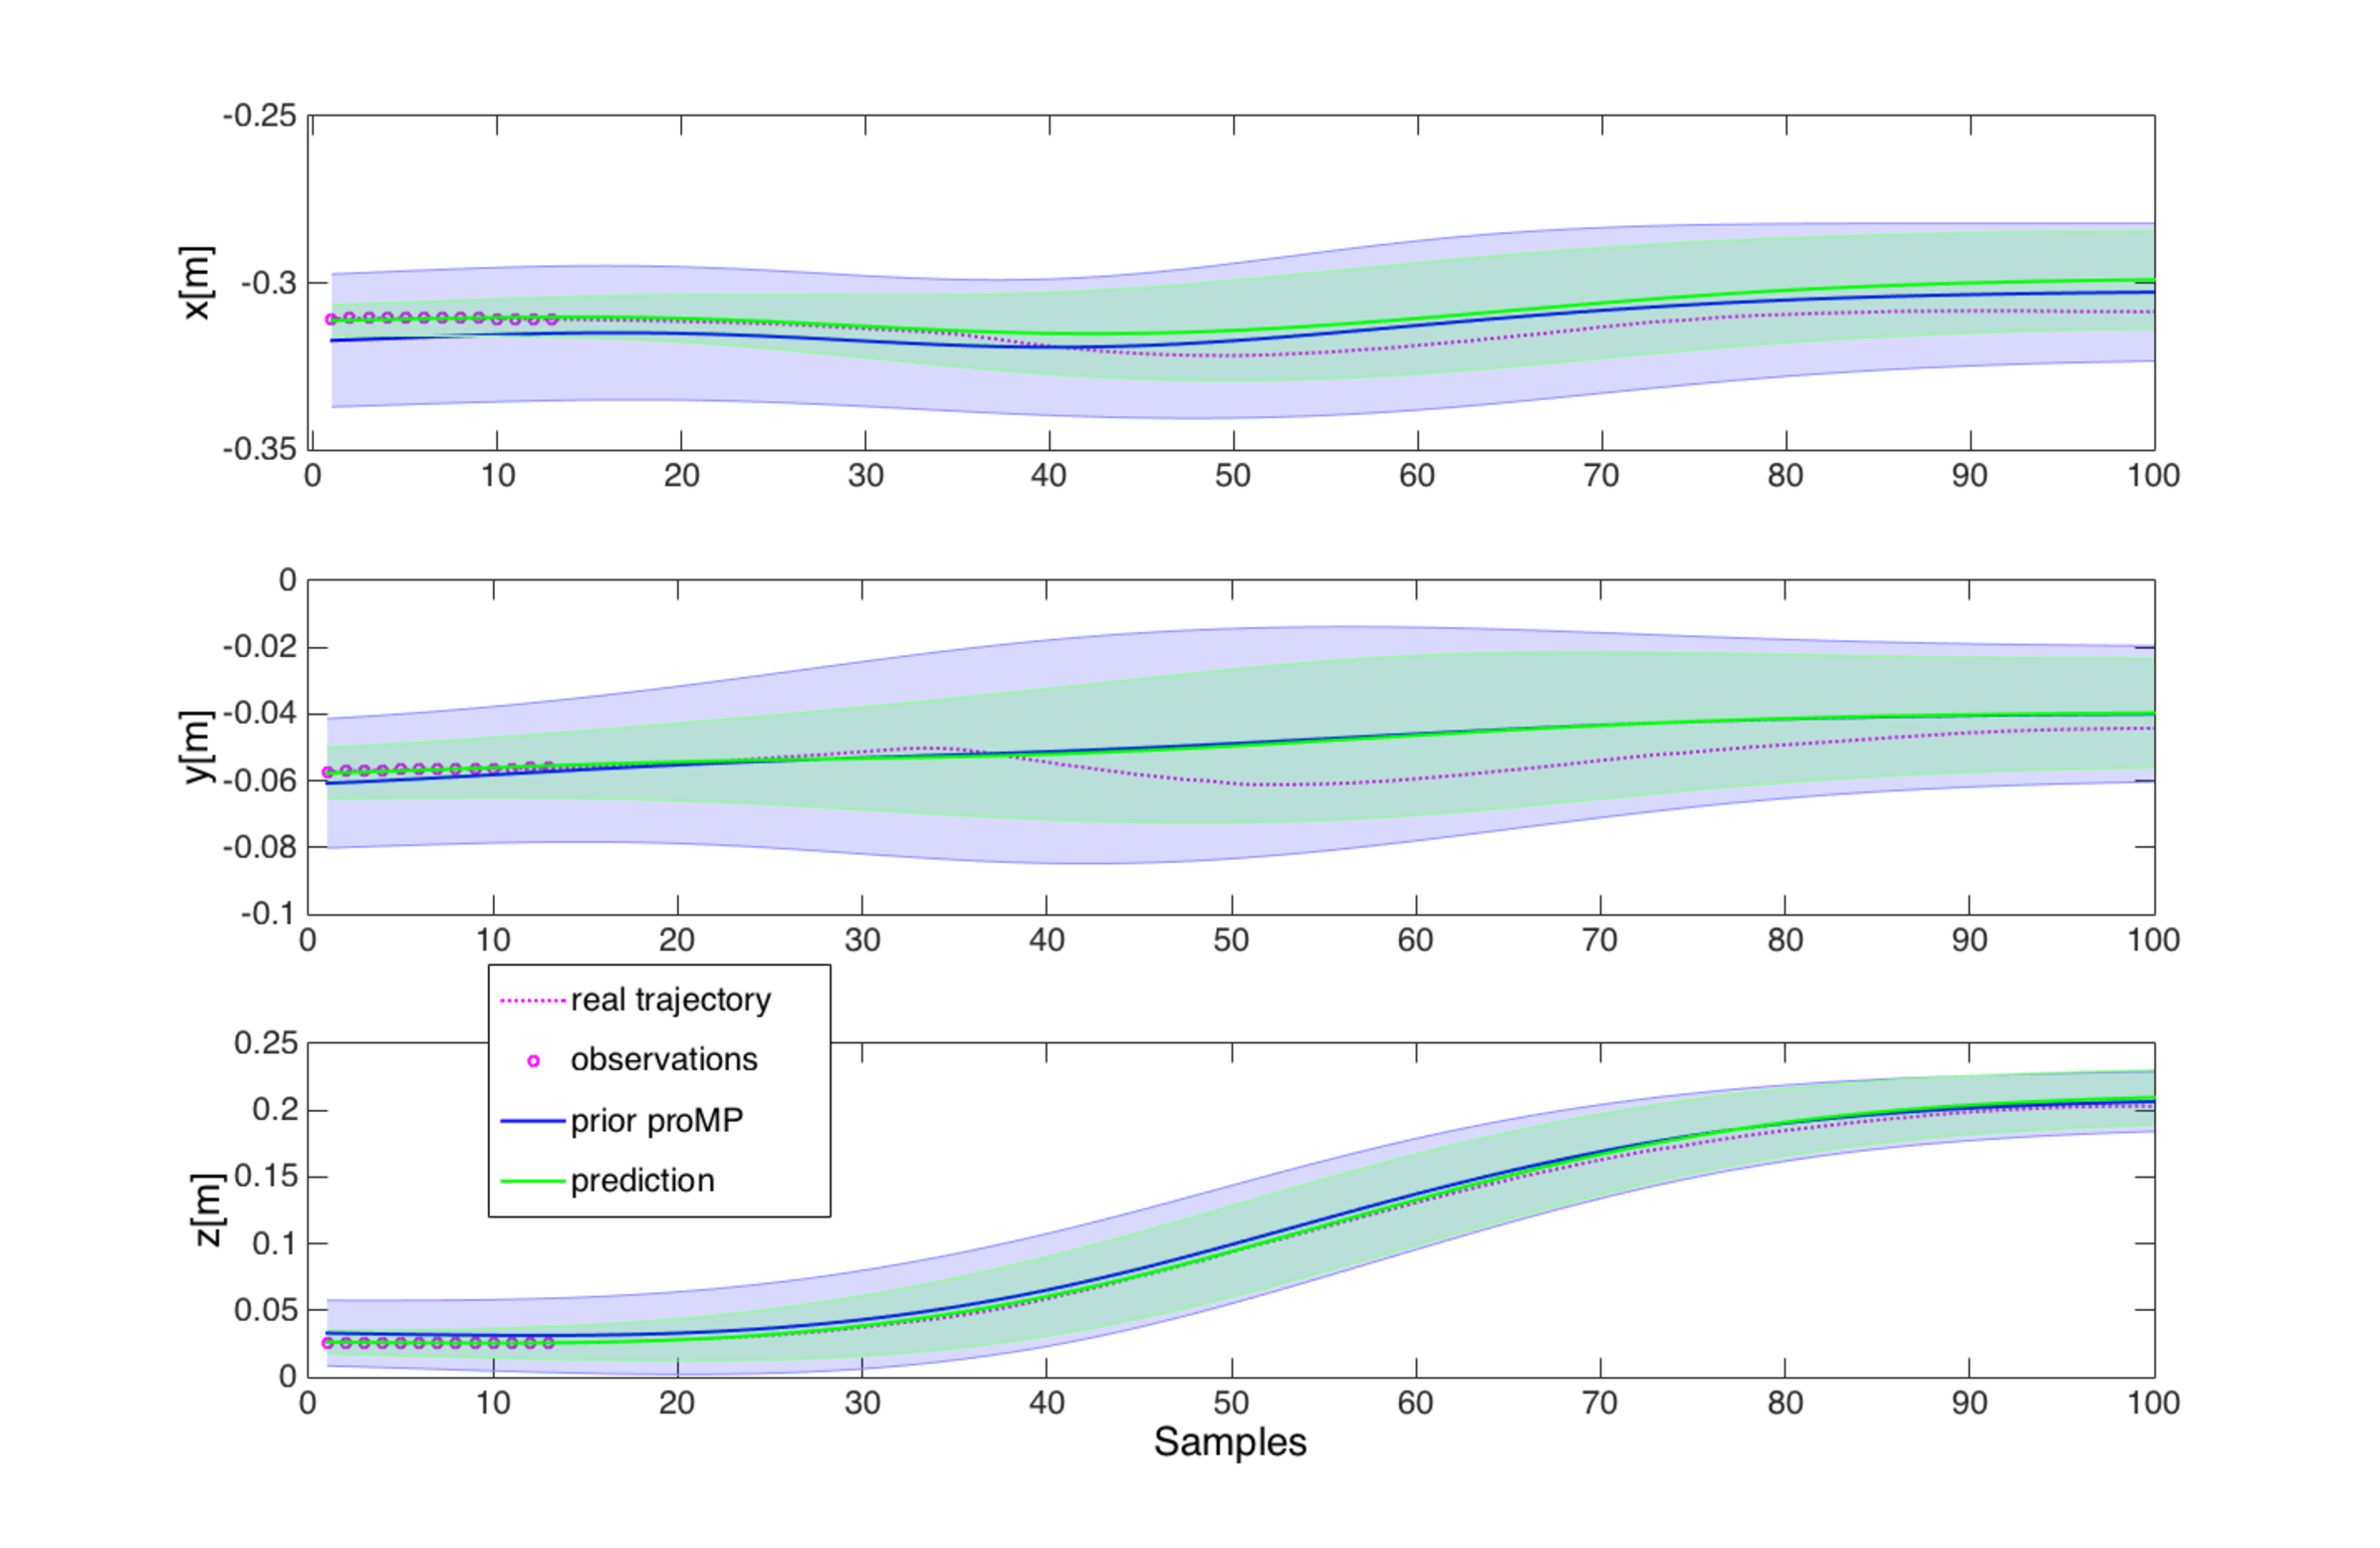
\includegraphics[height=11cm]{figs/proMP_prediction.pdf}
\caption{Prediction of the future trajectory, after $n_o=15$ observations, given the prior proMP learned from $n$ demonstrations.}
\label{fig:predictionLifting15}
\end{figure}










%!TEX root = ../D5.4.tex

\section{Conclusions and Future Works}
%
This report presents the progresses towards the implementation of 
learning how to stand up with the help of a human caregiver.
Presented results focus on: (1) human dynamics estimation while is physically 
interacting with a robot; (2) robot motion control for unassisted standing up 
motions. 

Human dynamics estimation is of pivotal importance
for a control design aimed at considering the \emph{human in the loop}
during physical human robot interaction. 
It provides in real-time the robot with the human force feedback
that could be used either as a tool for \emph{reactive} human-robot collaboration
(implying a robot reactive control) and, in a long-term perspective,
for \emph{predictive} collaboration, for enhancing remarkably the interaction naturalness.
Thus, the next step consists in developing a controller to endow the 
robot with the ability to adapt and adjust the interaction strategy.

 
 
 
 
 
 
 
 
 
 
  
  


\bibliographystyle{abbrv}
\bibliography{D5.4}
\end{document}

%%% Local Variables:
%%% mode: latex
%%% TeX-master: t
%%% save-place: t
%%% End:
